% !TeX program = xelatex
\documentclass[12pt,a4paper]{report}
\usepackage{fontspec}
\IfFontExistsTF{Times New Roman}{\setmainfont{Times New Roman}}{\setmainfont{TeX Gyre Termes}}
\IfFontExistsTF{Sylfaen}{\newfontfamily\georgianfont{Sylfaen}}{\IfFontExistsTF{Noto Serif Georgian}{\newfontfamily\georgianfont{Noto Serif Georgian}}{\newfontfamily\georgianfont{Arial Unicode MS}}}
\usepackage{polyglossia}
\setdefaultlanguage{english}
\setotherlanguage{georgian}
\usepackage[a4paper,left=3cm,right=1.5cm,top=2.5cm,bottom=2.5cm]{geometry}
\usepackage{setspace}
\onehalfspacing
\usepackage{booktabs}
\usepackage{graphicx}
\usepackage{caption}
\usepackage{float}
\usepackage{array}
\usepackage{amsmath}
\usepackage{siunitx}
\usepackage{pgfplots}
\pgfplotsset{compat=1.18}
\usepackage{tikz}
\usetikzlibrary{arrows.meta,positioning,calc}
\usepackage{chngcntr}
\counterwithout{figure}{chapter}
\counterwithout{table}{chapter}
\usepackage{hanging}
\usepackage{hyperref}
\usepackage{xcolor}
\usepackage{url}
\sisetup{detect-weight=true, detect-family=true, group-separator={,}, group-minimum-digits=4}
\captionsetup{font=small,labelfont=bf,justification=centering}
\hypersetup{colorlinks=true, linkcolor=black, citecolor=black, urlcolor=blue}
\setlength{\parindent}{1.25cm}
\setlength{\parskip}{0pt}
\setlength{\emergencystretch}{3em}
\renewcommand{\contentsname}{Table of Contents}
\makeatletter
\newcommand{\customtableofcontents}{\chapter*{Table of Contents}\@starttoc{toc}}
\makeatother
\DeclareRobustCommand{\code}[1]{\texttt{\detokenize{#1}}}
\begin{document}

\begin{titlepage}
\newgeometry{left=2.5cm,right=2.5cm,top=2.2cm,bottom=2.2cm}
\thispagestyle{empty}
\centering
\vspace*{0.3cm}

\includegraphics[width=0.18\textwidth]{figures/ibsu_logo.png}\par
\vspace{0.25cm}
{\bfseries International Black Sea University\\[-0.05em]School of Computer Science and Architecture\\[-0.05em]Computer Science\par}
\vspace{3.1cm}
{\bfseries\Large Morpheus: A Semantic Analysis System for\\[0.25em]Subconscious Data\par}
\vspace{3.7cm}
{\bfseries Ana Merabishvili\\Bachelor\textquotesingle{}s Thesis in Computer Science\par}
\vspace{4.1cm}
\begin{flushright}
{\bfseries Supervisor:\\Anri Morchiladze\par}
\end{flushright}
\vfill
{\bfseries Tbilisi, 2026\par}
\restoregeometry
\end{titlepage}
\pagenumbering{roman}
\customtableofcontents
\clearpage
\chapter*{Acknowledgements}
\addcontentsline{toc}{chapter}{Acknowledgements}
I would like to express my gratitude to my supervisor, Anri Morchiladze, for his guidance and feedback throughout the development of this bachelor\textquotesingle{}s thesis. I also thank the academic community of International Black Sea University for providing the institutional context in which this work could be developed, and my family and friends for their support during the research and implementation process.
\chapter*{Abstract}
\addcontentsline{toc}{chapter}{Abstract}
This thesis presents Morpheus, a semantic analysis system for transforming spoken and written dream narratives into structured psychological data. The system records subconscious dream material as mathematical data so that it can be analyzed, compared, processed, and visualized over time. As an intended baseline layout, Morpheus integrates local speech-to-text transcription through OpenAI Whisper, personally identifiable information anonymization, Jungian entity extraction, vector embedding generation, Retrieval-Augmented Generation, and graph-based longitudinal visualization. Its psychoanalytic interpretation layer is grounded in a curated knowledge base containing the work of Carl Jung, Sigmund Freud, and other established psychological theorists. The research argues that generic large language models are insufficient for mental-health-adjacent dream analysis because they are prone to hallucination, lack reliable psychoanalytic grounding, and operate statelessly across sessions. Morpheus addresses these limitations through a FastAPI backend, Supabase and pgvector persistence, a curated psychoanalytic knowledge base, and domain-specific retrieval. Within this architecture, Georgian Automatic Speech Recognition (ASR) is treated as a heavily constrained baseline target path under low-resource acoustic conditions and strict cloud memory and CPU limits. The empirical technical verification layer therefore uses dream-register English inputs to validate the downstream pipeline systematically, including anonymization, entity extraction, vector persistence, retrieval, and generated analysis. This separation preserves the system\textquotesingle{}s architectural claim without overstating raw Georgian audio readiness. It also defines a practical bridge toward low-cost domain adaptation, especially fine-tuning Whisper Base or Small on Georgian acoustic datasets using commodity GPU resources such as T4-class hardware. The thesis further proposes a psychometric framework for future human-impact validation based on Dream Recall Frequency, Lexical Density, the LuCiD scale, and intra-user semantic clustering.
\chapter*{\textgeorgian{ანოტაცია}}
\addcontentsline{toc}{chapter}{\textgeorgian{ანოტაცია}}
\begin{georgian}
ნაშრომში წარმოდგენილია ქვეცნობიერი ინფორმაციის, კერძოდ, სიზმრების, სემანტიკური ანალიზის სისტემა Morpheus. სისტემა მონაცემთა დამუშავებისთვის ეფუძნება სტრუქტურირებულ მეთოდოლოგიას, რომელიც უზრუნველყოფს ქვეცნობიერი ჩანაწერების მათემატიკურ წარმოდგენად გარდაქმნას, რაც შესაძლებელს ხდის მათ სიღრმისეულ ანალიზს, შედარებასა და დამუშავებას.

სისტემის სამუშაო პროცესი რამდენიმე ეტაპისგან შედგება. მომხმარებლის მიერ მოწოდებული აუდიოჩანაწერი OpenAI Whisper-ის მეშვეობით გარდაიქმნება ტექსტად, რის შემდეგაც ხდება სენსიტიური მონაცემების ავტომატური ანონიმიზაცია. მომდევნო ეტაპზე Retrieval-Augmented Generation (RAG) არქიტექტურის გამოყენებით ხორციელდება სიზმრის ფსიქოანალიტიკური ინტერპრეტაცია, რომელიც ეფუძნება კარლ იუნგის, ზიგმუნდ ფროიდისა და სხვა აღიარებული მკვლევრების ფსიქოლოგიურ ნაშრომებს. აღნიშნული პროცესი საშუალებას იძლევა გამოვლინდეს სიზმრის ძირითადი სიმბოლოები და ემოციური მდგომარეობები. მიღებული ინფორმაცია ვექტორული წარმოდგენით ინახება მონაცემთა ბაზაში და საბოლოოდ მომხმარებელს გრაფზე დაფუძნებული ვიზუალიზაციის სახით მიეწოდება.

ნაშრომი აჩვენებს, რომ Large Language Models (LLMs) დამოუკიდებლად არ არის საკმარისი სიზმრების ფსიქოლოგიური ანალიზისთვის, რადგან მათ ახასიათებთ ჰალუცინაციები, არ გააჩნიათ საკმარისი სპეციალიზებული ცოდნის ბაზა და ვერ ინარჩუნებენ გრძელვადიან კონტექსტს სესიებს შორის. Morpheus აღნიშნულ შეზღუდვებს გადალახავს FastAPI-ზე დაფუძნებული backend ინფრასტრუქტურის, Supabase პლატფორმის, pgvector-ის ვექტორული გაფართოებისა და სპეციალურად შერჩეული ფსიქოანალიტიკური ცოდნის ბაზის ინტეგრაციით.

სისტემის ტექნიკური შეფასება და ვერიფიკაცია ადასტურებს, რომ წარმოდგენილი არქიტექტურა მაღალეფექტიანია. ნაშრომში ასევე წარმოდგენილია გრძელვადიანი კვლევის დეტალური გეგმა, რომელიც სისტემის პრაქტიკულ ღირებულებას შეაფასებს წინასწარ განსაზღვრული მეტრიკების საფუძველზე. აღნიშნულ მეტრიკებს შორისაა სიზმრების გახსენების სიხშირე, ლექსიკური მრავალფეროვნება, LuCiD სკალა და მომხმარებლის ქვეცნობიერი ინფორმაციის შინაარსობრივი კლასტერიზაცია.
\end{georgian}
\clearpage
\pagenumbering{arabic}
\chapter*{Introduction}
\addcontentsline{toc}{chapter}{Introduction}
The systematic analysis of human inner experience has long occupied a peripheral position within computational research, with dream cognition representing perhaps the most underexplored dimension of that domain. Mental health informatics has made considerable advances in affective computing, sentiment detection, and clinical decision support over the past decade. Dream content, however, resists these frameworks. It is ephemeral, symbolically dense, and culturally encoded in ways that standardized diagnostic instruments rarely accommodate. The predominant methods for capturing dream data remain manual journaling and retroactive clinical interviews, both of which impose fundamental limitations on the quality of the data they produce. Recall bias distorts the fidelity of narratives recovered hours or days after waking, and the interpretive labor required of clinicians restricts the scale at which longitudinal analysis can be conducted. Temporal distortion compounds this problem further, as the affective weight and symbolic content of a dream shift in memory even within a single waking hour. These limitations are not incidental. They are structural features of analog collection methods that, uncorrected, render pattern detection across a patient\textquotesingle{}s dream history methodologically unreliable.

Morpheus addresses this structural problem directly. Morpheus is a semantic analysis system designed to automate the transformation of spoken or written dream narratives into structured psychological data that can be stored, queried, and analyzed at scale. Its conceptual architecture is engineered around a targeted Georgian ingestion blueprint in which spoken dream material is normalized, transcribed or translated through a local Whisper baseline, and routed into a multi-stage pipeline for entity extraction, embedding generation, and psychologically grounded interpretation. Framed this way, the ingestion layer establishes a structural baseline for low-resource, low-tier cloud deployment rather than a final claim about acoustic optimality. The foundational precedent for applying natural language processing to dream content at this level of semantic granularity is established by Saleemi (2025) in \textquotedbl{}Developing an AI Model for Dream Interpretation Based on Subconscious Analysis,\textquotedbl{} which demonstrates that Natural Language Processing (NLP)-based classification pipelines can reliably identify thematic and emotional categories within dream text. Morpheus extends that precedent considerably, treating classification not as an endpoint but as a preliminary step within a richer analytical architecture.

What distinguishes Morpheus from prior classification-based approaches is its implementation of a Retrieval-Augmented Generation (RAG) architecture grounded in Jungian and psychoanalytic source texts. Rather than mapping dream content to predefined label categories, the system retrieves semantically relevant passages from an academic knowledge base at query time, constructing a contextually enriched prompt that guides the language model toward evidence-based, theoretically coherent interpretation. The result is a mode of analysis that reflects the interpretive depth of clinical commentary rather than the categorical output of a classifier. This architectural choice has direct implications for the quality and defensibility of the psychological insights the system produces, particularly in the context of longitudinal tracking, where accumulated errors in early-stage classification can propagate and distort downstream pattern recognition.

The present research is oriented around two central questions that together define the scope of what Morpheus is designed to test. The first is whether a RAG-based pipeline, operating on a vector knowledge base of psychoanalytic literature, can produce semantically coherent and psychologically grounded analyses of dream content when applied at scale across diverse narrative inputs. The second concerns the feasibility of tracking latent emotional patterns, including anxiety, stress, and perfectionism, longitudinally through the geometric relationships that emerge in a high-dimensional vector space, where dreams sharing underlying affective content cluster in proximity regardless of their surface-level narrative differences. These questions are not independent. The validity of longitudinal pattern detection depends on the interpretive quality established at the single-dream level, and the system\textquotesingle{}s capacity to address both simultaneously constitutes its primary claim to methodological novelty.

The argument is developed across two chapters. Chapter 1 situates Morpheus within the broader landscape of computational psychology, surveying the engineering frameworks that have been applied to subconscious data tracking and examining in detail the limitations that generic large language models exhibit when deployed in mental health contexts without domain-specific grounding, before presenting a comprehensive account of the Morpheus architectural design, its backend infrastructure, and the rationale for the specific technical choices made at each stage of the pipeline. Chapter 2 then turns to the empirical dimensions of the project, beginning with a detailed treatment of document ingestion and text sanitization, tracing the construction of the vector embedding space, and evaluating the system\textquotesingle{}s technical performance under realistic operating conditions. Whereas Chapter 1 establishes the theoretical and architectural foundation, Chapter 2 concludes by proposing a psychometric framework and experimental design through which the clinical validity of the system\textquotesingle{}s outputs could be formally assessed in future research. Together, these chapters present Morpheus not simply as a working software system but as a rigorous methodological contribution to the nascent field of computational dream analysis.

\chapter{Computational Psychology and System Architecture}
The intersection of computational systems and psychological data presents a class of design problems that is qualitatively distinct from those encountered in conventional software engineering. Architecture is not neutral in this domain. The structural choices made at the level of data representation, model selection, and retrieval strategy directly determine the scientific validity of every output the system produces, and understanding why Morpheus was designed as it was therefore requires situating those decisions within a broader account of how computational approaches to psychological language have evolved and where earlier frameworks have failed.

\section{Engineering Frameworks for Subconscious Data Tracking}
Within the context of computational systems, \textquotedbl{}subconscious data\textquotedbl{} refers to unstructured, high-variance natural language generated from internal psychological states, as distinct from the structured behavioral or biometric signals that dominate adjacent fields such as physiological monitoring or activity tracking. A heart rate reading carries a precisely bounded meaning within a well-defined measurement schema. A dream narrative does not. Subconscious data encodes multiple emotional valences simultaneously, operates through symbol and metaphor rather than direct referential statement, and resists any schema that presupposes stable relationships between surface-level linguistic features and underlying psychological meaning. This fundamental property has defined both the ambitions and the persistent failures of every computational framework that has attempted to process it systematically.

The earliest efforts to analyze psychological language through computational means relied on keyword matching and rule-based sentiment classifiers, architectures that assigned emotional polarity to text by scanning for the presence of pre-categorized lexical items. The Linguistic Inquiry and Word Count system developed by Pennebaker et al. (2001) represents the most widely adopted instantiation of this approach, mapping word frequencies onto psychological dimensions through a manually curated dictionary of several thousand entries. These frameworks produced interpretable outputs and enabled a substantial body of quantitative research in personality psychology and clinical linguistics, but they introduced a critical and largely unacknowledged distortion. By reducing the affective content of natural language to binary or categorical polarity scores, they stripped precisely the complexity that makes psychological data scientifically valuable. A dream in which water appears as a symbol of suffocation and a dream in which water signals liberation would receive identical or near-identical scores under any keyword-frequency model, because the semantic relationship between a symbol and its psychological valence is not a function of the symbol\textquotesingle{}s presence alone. It is a function of the surrounding narrative context, the emotional register of the sentences that precede and follow it, and the theoretical framework through which the symbol is being interpreted. That contextual structure is exactly what rule-based systems cannot represent.

The emergence of transformer-based architectures fundamentally changed what was computationally achievable in natural language understanding. Devlin et al. (2019) introduced BERT, a bidirectional encoder that learns deep contextual relationships between tokens through masked language modeling on large text corpora, producing dense vector embeddings in which proximity in the representational space corresponds to proximity of meaning across the full surrounding context rather than within a fixed window. This capacity for contextual representation, extended through the generative turn inaugurated by models such as GPT, created the conditions under which a retrieval-augmented approach to psychological interpretation becomes not only viable but architecturally well-motivated. This property proved consequential for psychological language processing. For the first time, a model could represent the difference between \textquotedbl{}falling\textquotedbl{} as a physical event description and \textquotedbl{}falling\textquotedbl{} as an anxiety marker without requiring that distinction to be hand-coded by a researcher. The GPT family of autoregressive architectures extended the capabilities of transformer representations further by demonstrating that models trained at sufficient scale could generate semantically coherent, tonally appropriate continuations of complex and metaphorically dense text. The most directly relevant application of these capabilities to dream analysis is documented by Saleemi (2025), who applied BERT-based classification to a corpus of dream narratives and successfully categorized dominant emotional content into anxiety, sadness, and happiness clusters with measurable predictive accuracy. That work established the empirical feasibility of transformer-based approaches to the dream domain and constitutes the immediate NLP precedent that the Morpheus system extends and deepens.

The specific engineering challenge that differentiates psychological language processing from other NLP domains, however, is one that transformer classification alone cannot resolve. Psychological language is non-linear, metaphorical, and temporally recursive in ways that distinguish it categorically from news articles, product reviews, or the social media posts on which most NLP benchmarks are calibrated. A dream narrative may reference a childhood memory, a present anxiety about professional performance, and an imagined future scenario within three consecutive sentences, with no syntactic marker distinguishing one temporal plane from another. Standard classification pipelines fail under these conditions because they treat each input as a stateless event, encoding it as a fixed-dimension vector without any mechanism for grounding the interpretation in the established theoretical frameworks that give psychological symbols their diagnostic meaning. The Hall and Van de Castle (1966) quantitative coding system, which remains the foundational instrument for systematic dream content analysis in the psychological literature, made this requirement explicit at the empirical level decades before computational methods became sophisticated enough to address it. Their nominal coding categories, covering aggression, friendliness, sexuality, misfortune, and success, were not arbitrary. They were derived from psychoanalytic and depth psychology theory, and their predictive validity across cross-cultural studies depended precisely on that theoretical anchoring. A computational system that discards this grounding in favor of purely data-driven pattern recognition loses the interpretive validity that clinical analysis requires.

Retrieval-Augmented Generation addresses this structural problem at the architectural level. Lewis et al. (2020) introduced the RAG framework as a method for combining a parametric generative language model with a non-parametric retrieval mechanism operating over an external document store, enabling the model to condition its generated outputs on retrieved passages of domain-specific evidence at inference time, rather than relying solely on knowledge encoded in model weights during pre-training. The implications for psychological language analysis are immediate. A RAG system can be configured so that every interpretation is conditioned on retrieved passages from domain-specific theoretical literature. This ensures that outputs reflect not only what the language model can infer from the dream text alone, but also what established psychoanalytic frameworks indicate about the symbols and emotional configurations present in the narrative. In Morpheus, this knowledge store is constituted by a curated corpus of psychoanalytic and depth psychology texts maintained in the books directory of the backend repository. At query time, a cosine similarity search over the \code{knowledge_base} table in Supabase retrieves the most semantically proximate passages from this corpus and injects them into the generative prompt as theoretical context, before the language model produces its analysis. Domain-specific grounding of this kind is not merely a design preference in mental health applications. It is a scientific necessity, because a system that produces interpretations that are linguistically fluent but theoretically unanchored creates the appearance of clinical validity without its substance, a failure mode that is arguably more consequential than producing no interpretation at all.

Establishing this engineering foundation clarifies the specific shortcomings that arise when generic, off-the-shelf language models are deployed in mental health contexts without the domain-specific retrieval scaffolding that Morpheus implements, and those shortcomings are what Section 1.2 addresses directly.

\section{Limitations of Generic Large Language Models in Mental Health}
General-purpose large language models, including GPT-4, Claude, and the Llama family of open-weight models, represent a remarkable advance in the capacity of computational systems to produce fluent, contextually appropriate natural language across an extraordinarily wide range of topics and tasks. Their outputs are coherent, their tone is adjustable, and their apparent comprehension of complex subject matter is, in many domains, functionally indistinguishable from that of a knowledgeable human reader. This fluency, however, is not the same property as validity. In most application domains, the gap between the two is tolerable. A general-purpose model that produces a slightly imprecise summary of a news article causes no meaningful harm. In clinical and psychological contexts, the gap between fluency and validity is not tolerable at all. It is consequential in ways that require careful architectural attention.

The most structurally significant failure mode of large language models in mental health applications is hallucination. Language models generate outputs by sampling from probability distributions over possible token sequences conditioned on the preceding context. They do not verify claims against ground truth before producing them. When a model has insufficient grounding in the specific domain it is being asked to reason about, it produces outputs that are syntactically and stylistically convincing but factually or theoretically unsupported, a phenomenon consistently documented in the literature on large language model (LLM) reliability (Maynez et al., 2020). In the context of dream analysis, a hallucinated interpretation is not merely an error in the conventional software sense. If a user receives a fluent, confident psychological reading of their dream that attributes to them an emotional pattern or psychological tendency that the model generated without valid theoretical basis, and if that user internalizes it as insight, the harm is direct and not hypothetical. This is not a risk specific to any single model or provider. It is a structural consequence of the generation mechanism itself, and it cannot be corrected by prompt engineering alone.

The knowledge boundary problem compounds the hallucination risk considerably. Large language models are trained on internet-scale corpora in which psychologically relevant content is present but thoroughly diluted by pop-psychology articles, self-help blog posts, journalistic interpretations of therapeutic concepts, and layperson accounts of dreams and emotional experiences. Within that training distribution, the signal representing rigorous Jungian or psychoanalytic frameworks, including the theoretical constructs of the collective unconscious, shadow integration, anima and animus dynamics, and individuation, is vanishingly small relative to the noise. The model consequently has no reliable internal representation of these frameworks as theoretical systems. It can produce text that uses the vocabulary of depth psychology fluently, because that vocabulary appears in its training data, but it cannot be expected to apply the frameworks with the consistency and precision that clinical interpretive validity requires. Generic fluency with psychoanalytic terminology is not the same as theoretical grounding, and the difference between the two is precisely what determines whether an interpretation has scientific standing.

A further limitation that is rarely foregrounded in general NLP discussions but is critical in psychological applications is the statelessness of standard language model deployments. Each call to a commercial language model Application Programming Interface (API) is contextually isolated. The model receives no information about prior sessions, retains no record of the emotional content the user has described across previous interactions, and has no capacity to construct a longitudinal picture of the user\textquotesingle{}s psychological state. For a single-session creative writing assistant, this property is irrelevant. For a system intended to track whether anxiety markers in a user\textquotesingle{}s dream journal are becoming more frequent, more intense, or clustering around specific symbolic motifs over thirty days, statelessness is a fundamental architectural disqualification. No amount of prompt augmentation within a single API call can substitute for a persistent, queryable record of prior semantic content, because the analytical value of longitudinal tracking lies precisely in the relationships between sessions rather than within any single one.

The ethical dimension of commercial API dependency in mental health applications demands separate consideration. Dream content is among the most intimate categories of personal psychological data a user can generate. Routing that content through third-party infrastructure, including the inference endpoints of commercial model providers, exposes it to data retention policies, model fine-tuning pipelines, and security surfaces that the user cannot audit or control. This concern applies regardless of the specific privacy commitments made by any given provider, because the structural exposure exists at the level of transmission and processing rather than at the level of contractual intent. Mental health informatics applications have an obligation to minimize unnecessary data movement, particularly when local and privacy-preserving alternatives exist.

Morpheus is designed with each of these limitations in explicit view. The knowledge boundary problem is addressed through the domain-specific \code{books} corpus, which supplies the psychoanalytic grounding that the generative model itself cannot be assumed to possess reliably, ensuring that every produced interpretation is conditioned on retrieved passages from established theoretical literature rather than on training data of uncertain provenance. The longitudinal limitation is addressed through persistent vector storage in Supabase, where every processed dream is saved as a \num{384}-dimensional embedding alongside its extracted metadata, enabling session-to-session semantic comparison across the full duration of a user\textquotesingle{}s engagement with the system. The privacy concern is addressed through local embedding computation via \code{sentence-transformers}, which processes all dream text on the application\textquotesingle{}s own infrastructure rather than transmitting it to a commercial embedding API. It is worth observing that the BERT-based classification approach taken by Saleemi (2025), by forgoing generation entirely in favor of discriminative classification, sidestepped the hallucination problem altogether, and that architectural conservatism was appropriate and defensible for the research scope they defined. The limitation of that approach is that discriminative classification, however accurate, cannot produce the interpretive narrative depth that makes psychological analysis clinically useful rather than merely categorical. Extending their work to include generation is what introduces the hallucination risk, and the RAG architecture implemented in Morpheus is the mechanism through which that risk is controlled.

\section{Morpheus Architectural Design and Backend Infrastructure}
Morpheus is a Progressive Web Application (PWA). Its architecture splits across three distinct layers, each assigned a different class of operations. The user-facing layer handles input capture, real-time state presentation, and graph-based visualization. Request coordination, validation enforcement, and service routing belong to the API layer. Persistence, vector search, and language model inference live in the combined data and intelligence layer. None of these separations were accidental. By keeping the intelligence layer decoupled from the API layer, individual service components can be evaluated, replaced, or upgraded independently. This applies to the speech-to-text module, the embedding model, and the language model client alike. Swapping any one of them out does not disrupt the broader application.

Python 3.11 powers the backend. FastAPI serves as the web framework, with Uvicorn running as the Asynchronous Server Gateway Interface (ASGI) server. Each of these choices connects directly to the application\textquotesingle{}s operational requirements. Through asynchronous request handling, FastAPI prevents I/O-bound operations from blocking concurrent requests. Database writes, embedding computation, and external language model API calls all qualify as such operations. For a pipeline that chains multiple sequential operations of variable latency, this matters enormously. Type-safe request and response validation is enforced through Pydantic schema models. This cuts the class of input-handling errors that can corrupt downstream analytical steps. OpenAPI documentation is generated automatically from type annotations. That produces a persistent, machine-readable record of the API contract. Both development verification and academic reproducibility standards benefit from it. Under the app directory, \code{main.py} defines the FastAPI application instance. \code{config.py} manages environment variable loading through Pydantic settings. \code{database.py} provides the Supabase client used across all persistence operations.

Two primary API endpoints define the system\textquotesingle{}s contract with its users. Each corresponds to a distinct phase of user interaction. \code{POST /v1/dreams/process} accepts an audio file upload and runs the full analytical pipeline in sequence. First, audio format conversion and speech-to-text transcription. Then personally identifiable information (PII) anonymization, Jungian entity extraction, and semantic embedding generation. After that, the RAG retrieval step executes, followed by psychological analysis. All outputs are then persisted to the database before the endpoint returns a structured response. \code{GET /v1/graph/data} works differently. It queries the dreams, keywords, and \code{dream_keywords} tables. A JavaScript Object Notation (JSON) structure comes back containing two arrays: one of nodes representing individual dream sessions and extracted keywords, the other of links representing relational connections between them. The frontend consumes this directly for graph rendering. Both endpoints appear simple at the interface level. That simplicity is a direct result of the complexity the service layer absorbs behind them.

The intended speech ingestion design relies on Whisper in translation mode, allowing Georgian dream narratives to be converted into English text before anonymization, symbolic extraction, embedding generation, and retrieval-based interpretation. This design reduces dependence on Georgian-specific downstream Natural Language Processing (NLP) components, while making the acoustic layer a deliberately visible baseline rather than an assumed solved component. Georgian presents a difficult operating condition for generalized speech recognition models because its Kartvelian structure, rich morphology, agglutinative patterns, and limited representation in large multilingual training corpora weaken zero-shot transcription quality, especially when speech is informal, emotional, or recorded under mobile conditions. In Morpheus, the first analytical stage therefore marks the baseline computational ceiling of open-weight multilingual speech models under strict memory and CPU limits. Local deployment remains justified, since psychological profile data stays isolated inside the application infrastructure, repeated transcription introduces zero per-call financial overhead, and the deployed model weights remain consistent with the commercial Whisper family. The same constraint also gives the project a technically coherent next step. Fine-tuning Whisper Base or Small on Georgian acoustic datasets is far cheaper than deploying medium or large models continuously, and it is realistic on commodity GPUs such as NVIDIA T4 instances.

Supabase underpins the persistence layer. It combines a managed PostgreSQL instance with the \code{pgvector} extension for high-dimensional vector storage and cosine similarity search. Four tables organize the schema, each with cleanly separated responsibilities. The dreams table stores the raw transcribed text, the generated psychological analysis, and the \num{384}-dimensional embedding vector for each processing session. User identity and timestamp metadata are stored alongside these. The keywords table maintains a deduplicated registry of all extracted psychological terms. Because of this, the same symbol encountered across multiple dream sessions maps to a single node in the relational graph rather than creating redundant duplicates. Many-to-many relationships between individual dream sessions and their associated keywords are encoded in the \code{dream_keywords} junction table. This relational structure is what the graph visualization endpoint traverses. Chunked and embedded passages from the psychoanalytic source texts in the books directory are stored in the \code{knowledge_base} table. A stored database procedure named \code{match_documents} runs cosine similarity search over this table at query time. It accepts a query embedding and returns the top-k most semantically similar passages. These passages form the RAG context injected into the analysis prompt.

Railway hosts the backend. The backend repository defines deployment configuration through three files: \code{Procfile}, \code{nixpacks.toml}, and \code{requirements.txt}. Cloud deployment carries architectural significance beyond operational convenience. Dream recall peaks during the hypnopompic state. This is the brief transitional window between sleep and full wakefulness. During this window, narrative memory of a dream remains accessible before consolidation degrades it. A system requiring a locally running laptop to be powered on and initialized simply cannot serve that moment. By keeping the backend continuously available from any networked device, including a phone held in bed, Railway deployment aligns the system\textquotesingle{}s availability model with the exact window of highest user data quality.




\begin{figure}[H]
\centering
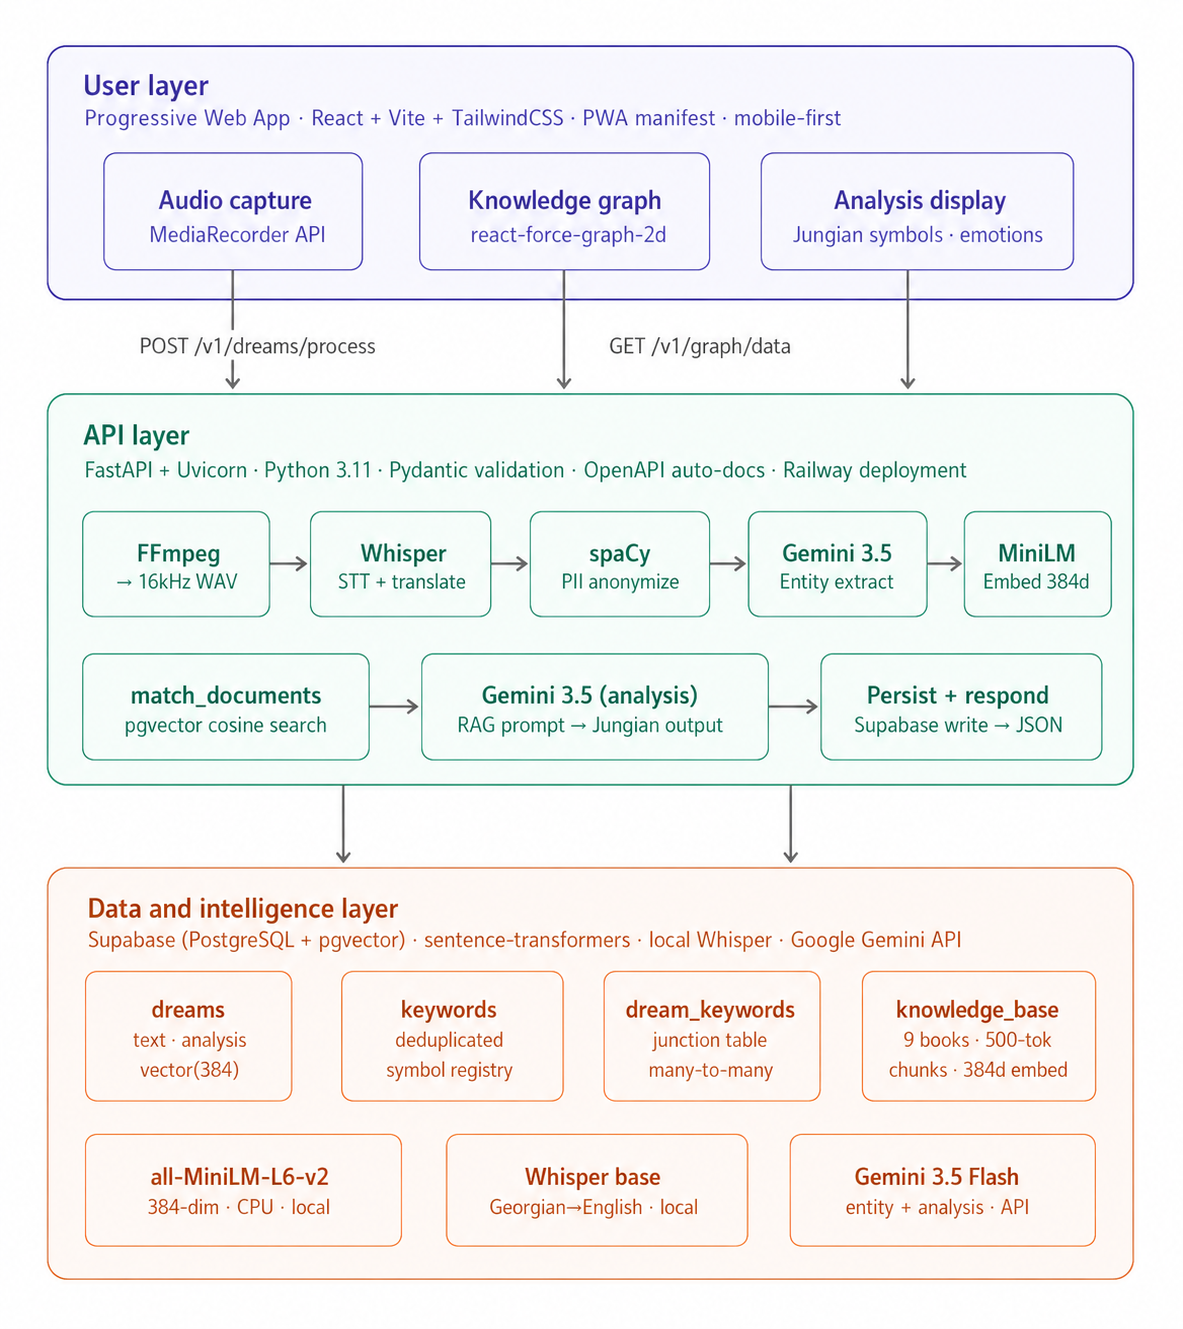
\includegraphics[width=0.96\textwidth,height=0.78\textheight,keepaspectratio]{figures/morpheus_system_architecture.png}
\caption{Morpheus system architecture. The diagram shows the user layer, API orchestration layer, and data and intelligence layer, including audio capture, graph display, FastAPI routing, FFmpeg normalization, Whisper transcription and translation, spaCy anonymisation, Gemini 3.5 Flash entity extraction and analysis, MiniLM embeddings, Supabase persistence, and pgvector-based knowledge retrieval.}
\label{fig:morpheus-three-tier-pipeline}
\end{figure}

React and Vite make up the frontend stack. TailwindCSS handles component styling. A mobile-first responsive layout governs the design, suited to the primary use context. At the center of the interface sits the knowledge graph, the application\textquotesingle{}s central visualization artifact. It renders through \code{react-force-graph-2d}, a D3-force-based library. Physics-simulated force-directed graph layouts emerge from it, where node positions are determined by the relational structure of the data rather than manual placement. A PWA manifest file configures the application for installation on mobile devices. Once installed, it launches from a home screen with no browser chrome. That removes friction between waking and capturing a dream narrative. Across every layer, every architectural decision in Morpheus targets the same goal: converting ephemeral subjective psychological experience into durable, queryable, semantically structured data. Enough meaning is retained in that structure to support longitudinal analysis.

\chapter{Data Engineering, Semantic Pipelines, and Empirical Evaluation}
Chapter 1 established the theoretical and architectural foundations of the Morpheus system. Chapter 2 turns to the operational substance of those foundations, examining in detail the data engineering pipeline that transforms raw psychological input into semantically structured knowledge, and the empirical methods used to evaluate both the system\textquotesingle{}s technical behavior and the validity of its psychological outputs. These two concerns are not separable, because the reliability of every downstream analytical claim depends directly on the quality of the data engineering decisions made upstream.

\section{Document Ingestion and Text Sanitization}
Morpheus faces two fundamentally different data ingestion problems. Conflating their requirements would compromise both. The first track handles real-time user input: audio recordings of dream narratives that arrive as live, variable-quality data and must be transformed into clean, anonymized, structured text before any psychological analysis can begin. The second track is different entirely. Static ingestion of academic and psychoanalytic source texts into the knowledge base is a one-time preprocessing operation, and its output quality determines every RAG retrieval the system will ever perform. Each track demands its own sanitization strategy. Describing them separately clarifies both the technical design and the reasoning behind it.

Audio capture for the user input track runs through the browser\textquotesingle{}s MediaRecorder API. The browser encodes the spoken dream narrative as a compressed audio blob and submits it to the FastAPI \code{POST /v1/dreams/process} endpoint as a multipart form upload. Format normalization is the first backend operation. Because browsers produce WebM, OGG, and MP4 files depending on operating system and vendor behavior, the service layer calls FFmpeg to convert each incoming file to a \SI{16}{\kilo\hertz} mono WAV before speech processing begins. This step gives the conceptual architecture a stable acoustic input format regardless of client device. In the intended baseline layout, speech-to-text processing then runs through the \code{openai-whisper} library as a locally loaded model instance (OpenAI, 2023). With \code{task=\textquotedbl{}translate\textquotedbl{}}, Whisper performs language detection and returns English text, which keeps the downstream anonymization, extraction, embedding, and retrieval stages language-agnostic. Georgian makes this choice both useful and technically demanding. Its Kartvelian phonetics, morphological density, and comparatively low representation in multilingual speech corpora mean that Whisper Base should be treated as a constrained baseline model under low-tier cloud deployment, not as the upper bound of the architecture. Local execution is still the correct starting point because sensitive psychological audio remains inside the application infrastructure, per-call transcription cost disappears, and the model family stays compatible with later adaptation. The empirical findings in Section 2.3 therefore follow naturally from the design rather than contradicting it, since the baseline layout validates the pipeline while Georgian-specific fine-tuning of Whisper Base or Small offers the budget-conscious route toward stronger acoustic performance.

\begin{figure}[H]
\centering
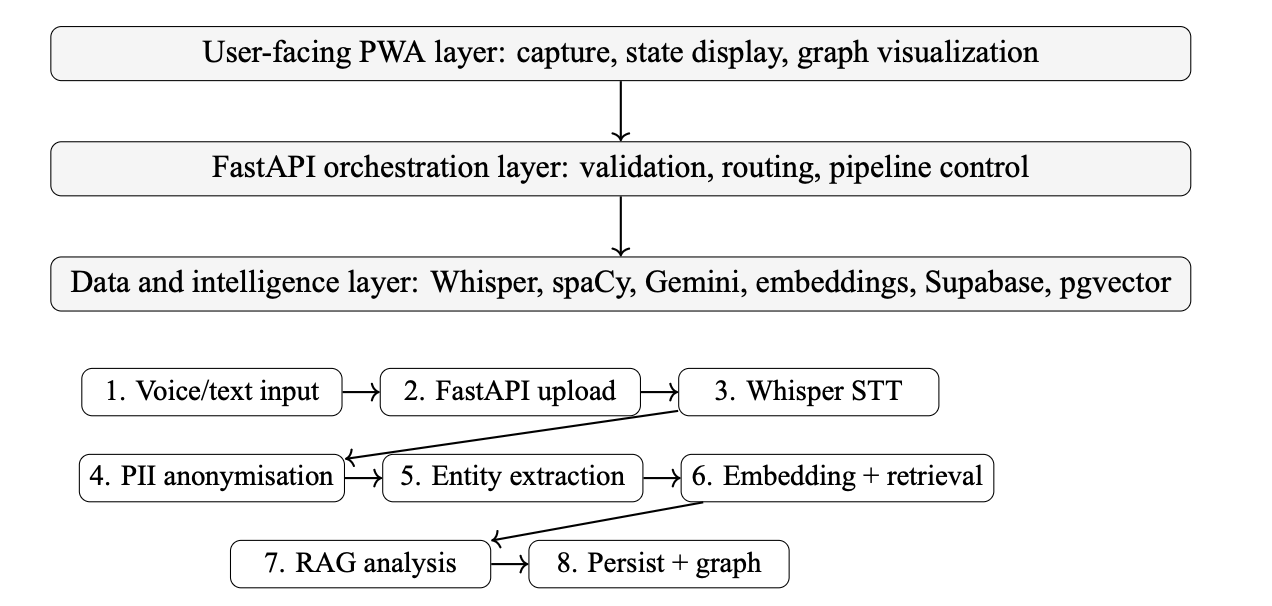
\includegraphics[width=0.96\textwidth]{figures/pipeline_chart.png}
\caption{Operational pipeline chart for the Morpheus processing sequence. The chart summarizes the layered control flow from the user-facing PWA through FastAPI orchestration and into the data and intelligence layer, followed by the eight-step processing path from voice or text input to persistence and graph construction.}
\label{fig:pipeline-chart}
\end{figure}

Before any further processing occurs, the raw transcript passes through a PII anonymization layer. Two levels of detection run here. A spaCy named entity recognition model identifies PERSON entities in the transcribed text and replaces each identified span with the placeholder token [PERSON], using a reverse-order substitution strategy that preserves character offsets across multiple replacements within the same string. On top of that, compiled regular expression patterns handle the remaining personally identifiable categories, replacing email addresses, phone numbers, and specific dates with the placeholder tokens [EMAIL], [PHONE], and [DATE] respectively. Choosing spaCy NER for person names rather than a regex approach directly targets a known failure mode of purely pattern-based anonymization: the mis-tagging of place names, organization names, and other capitalized tokens as personal identifiers. Why anonymization matters operates at two levels. Ethically, it prevents identifiable personal information from being associated with intimate psychological content in persistent storage. Technically, it strips tokens carrying no psychological signal from the text that Gemini 3.5 Flash processes in the next stage, reducing noise in the entity extraction output. That extraction runs in JSON mode, enforcing a strict schema requiring four fields: a short evocative dream title, an array of Jungian symbols, an array of dominant emotions, and a one-sentence narrative summary. Schema enforcement is not a convenience feature. It is a reliability guarantee. Without output constraints, a generative model can produce malformed, inconsistent, or hallucinated responses that silently corrupt downstream pipeline stages when parsed and persisted to the database.

Knowledge base ingestion, the second track, operates on eight psychoanalytic and depth psychology source texts that form the RAG retrieval corpus. These include Freud\textquotesingle{}s \textquotedbl{}The Interpretation of Dreams\textquotedbl{} (Freud, 2010), Jung\textquotesingle{}s \textquotedbl{}Archetypes of the Collective Unconscious\textquotedbl{} (Jung, 1981), \textquotedbl{}Man and His Symbols\textquotedbl{} (Jung, 1964), Campbell\textquotesingle{}s \textquotedbl{}The Hero with a Thousand Faces\textquotedbl{} (Campbell, 2008), Eliade\textquotesingle{}s \textquotedbl{}Myths, Dreams and Mysteries\textquotedbl{} (Eliade, 1960), Jung\textquotesingle{}s \textquotedbl{}Memories, Dreams, Reflections\textquotedbl{} (Jung \& Jaffe, 1989), and symbol dictionaries by Cirlot (2001) and Chevalier and Gheerbrant (1996). These files arrive from Project Gutenberg and other digital editions with uneven noise profiles. If the system ingests that material unchanged, retrieval quality falls quickly. The sanitization utility \code{clean_for_rag.py} addresses it through a multi-stage pipeline applied to each source file in sequence. Stage one strips Project Gutenberg legal wrappers, which bookend the actual text with license headers and footers carrying no psychological content and would otherwise inflate spurious retrieval matches. Stage two corrects Optical Character Recognition (OCR) artifacts introduced during digitization: soft hyphen line breaks splitting compound words across lines, year misreads where the digit 1 was scanned as the letter i producing strings such as i960 in place of 1960, and stray decorative Unicode symbols left over from the original typesetting. Stages three and four strip back matter and front matter respectively. Back matter removal targets index blocks, bibliography sections, footnote compilations, acknowledgment pages, and publisher marketing material, all of which carry dense but contextually decontextualized language that pollutes the semantic similarity space. Front matter removal targets copyright pages, ISBN lines, publisher addresses, endorsement quotes, and other boilerplate, using pattern-matching against known publisher identifiers combined with a heuristic that detects genuine prose onset by measuring paragraph length and sentence-ending density. Stage five removes tables of contents and illustration lists that survive front-matter stripping in texts with complex structural layouts. The final normalization stage collapses excessive whitespace, removes isolated page numbers and roman numeral page markers that OCR preserved as standalone lines, strips footnote superscript digits glued to adjacent word tokens, and eliminates table-of-contents leader dots and separator bars. For texts identified as alphabetical reference dictionaries, detected by the structural fingerprint of a standalone capital letter followed immediately by a lowercase entry word, an additional pass removes all-caps page-running headers that OCR introduced between dictionary entries.

Once the source texts are clean, the ingestion script applies sentence-aware segmentation rather than a fixed character-window split. The earlier fixed strategy used approximately \num{2000} characters with a \num{200}-character overlap, but the readiness audit showed that this approach split roughly \num{98} to \num{99} percent of chunks in the middle of sentences, introducing avoidable retrieval noise. The implemented chunker therefore first splits the full text at natural sentence boundaries: a period, exclamation mark, or question mark followed by whitespace and a capital letter. It then groups complete sentences into chunks that stay under \num{2000} characters and carries the last two sentences of each chunk into the next one as overlap. This keeps every retrievable unit anchored in complete prose. The overlap still matters, but it now preserves conceptual continuity without cutting through an argument or theoretical definition. Psychoanalytic concepts often unfold across several sentences, especially in discussions of archetypes, symbols, trauma, and myth; by overlapping the final two sentences, the system keeps those transitions visible to cosine similarity search. Each chunk is embedded with the same \code{all-MiniLM-L6-v2} sentence-transformer model used for dream embeddings, producing a \num{384}-dimensional vector. The ingestion script stores the resulting record in the Supabase \code{knowledge_base} table by mapping the cleaned filename to \code{book_title}, the chunk text to \code{content}, and the vector representation to \code{embedding}. In the completed ingestion run, this procedure produced exactly 6,209 chunks across eight cleaned texts. This metadata mapping gives each retrieved passage a clear source. Provenance is not cosmetic here. It is a basic requirement for academically defensible interpretation.

Before inserting records from any given source file, the ingestion script enforces a quality gate. It queries the \code{knowledge_base} table for existing entries sharing the same book title and skips ingestion entirely if matches are found. That deduplication check blocks the accumulation of redundant embedding vectors that would skew the cosine similarity distribution. Without it, passages from over-represented texts dominate retrieval results and cut the effective diversity of the knowledge base. With sanitization, chunking, and verified uniqueness in place, the embedding and retrieval pipeline determines how semantic meaning gets encoded and queried at inference time. Section 2.2 covers that.

\section{Vector Embeddings and Latent Theme Mapping}
An embedding is a function that maps a sequence of natural language tokens to a fixed-dimensional point in a continuous metric space, such that semantic similarity between input texts corresponds to geometric proximity between their representative points. This property is what makes embeddings useful for psychological language analysis. Two dream narratives that describe structurally different experiences but share an underlying emotional register, both involving confrontation with authority, both suffused with anticipatory anxiety, will produce embedding vectors that are close together in the representational space even if they share no surface vocabulary. The \code{sentence-transformers} model \code{all-MiniLM-L6-v2}, which generates all embeddings in the Morpheus system, produces a \num{384}-dimensional output space and is trained specifically to optimize semantic similarity tasks by fine-tuning on large-scale natural language inference and semantic textual similarity benchmarks (Reimers \& Gurevych, 2019). It is computationally lightweight enough to run without GPU acceleration on the Railway deployment infrastructure, which is a practical requirement given the memory constraints of the free-tier hosting environment, and its output dimensionality of 384 is sufficient to represent the semantic complexity of dream narratives while remaining tractable for cosine similarity search at the scale of a personal dream journal.

The choice of cosine similarity as the retrieval distance metric requires explanation before the formal definition is introduced. Embedding vectors vary in magnitude depending on the length and density of the text they represent. A one-sentence dream fragment and a six-sentence narrative describing the same core psychological experience will produce vectors of different magnitudes. A Euclidean distance metric would assign a larger separation to these vectors purely on the basis of that magnitude difference, misrepresenting their semantic proximity. Cosine similarity solves this problem by measuring the angle between two vectors rather than the absolute distance between their endpoints, normalizing for magnitude and capturing directional alignment in the embedding space. Two vectors pointing in the same direction receive a cosine similarity of 1 regardless of how long or short each vector is, while two vectors pointing in opposite directions receive a score of 0. For embedding-based retrieval over psychological text, where input length varies considerably and semantic relatedness should be the dominant signal, cosine similarity is the correct metric. The formula governing the computation is as follows.

\[
\cos(\theta) = \frac{\mathbf{A} \cdot \mathbf{B}}{\lVert\mathbf{A}\rVert\,\lVert\mathbf{B}\rVert}
\]
In this expression, $\mathbf{A}$ and $\mathbf{B}$ represent the \num{384}-dimensional embedding vectors of two texts being compared, the dot product in the numerator captures their directional alignment by summing the products of their corresponding components, and the product of their $L_2$ norms in the denominator normalizes the result to the interval between 0 and 1 for non-negative embeddings. In the Morpheus application context, $\mathbf{A}$ is the embedding of the incoming dream narrative, and $\mathbf{B}$ is the embedding of a stored chunk in the \code{knowledge_base} table, with the computation executed across the entire stored corpus to identify the passages most relevant to the user\textquotesingle{}s current dream content.

The \code{match_documents} stored procedure in Supabase implements this retrieval operation as a native database function using the \code{pgvector} extension. The procedure accepts a query embedding vector, a minimum similarity threshold, and a maximum result count as parameters. It computes the cosine similarity between the query vector and every stored knowledge base embedding using \code{pgvector}\textquotesingle{}s \code{<=>} cosine distance operator, converts the distance to a similarity score by computing \code{1 - distance}, filters out any result falling below the specified threshold, and returns the top-k remaining results ordered by descending similarity. The threshold filter is not a minor optimization. A generative language model will incorporate whatever context it receives into its output. If the retrieval step surfaces passages that are semantically distant from the dream content simply because no sufficiently similar passage exists in the knowledge base, the model will attempt to construct an interpretation from that irrelevant context, producing outputs that are fluent but analytically misleading. Enforcing a minimum similarity threshold means the generative prompt is either grounded in genuinely relevant theoretical material or left without retrieved context, both of which are preferable to grounding it in noise.

Latent theme mapping is the longitudinal function that distinguishes Morpheus from a single-session dream analysis tool. Each dream narrative processed by the system generates an embedding vector that is stored alongside its metadata in the \code{dreams} table. Over repeated sessions, the collection of a user\textquotesingle{}s dream embeddings defines a trajectory through the \num{384}-dimensional semantic space. The geometric structure of that trajectory, specifically the clustering patterns and directional tendencies within it, encodes information about the user\textquotesingle{}s recurring psychological preoccupations that the user may not have consciously identified or articulated. A set of dream embeddings that consistently cluster in a region of the embedding space associated with themes of evaluation by authority figures, performance failure, and urgency under constraint, themes that are representable in the Jungian knowledge base through passages on perfectionism, the shadow, and the animus dynamic, indicates a latent stress or perfectionism pattern. That inference does not require the user to have mentioned perfectionism in any single dream narrative. It emerges from the geometric distribution of the embeddings across sessions.

The graph data structure returned by the \code{GET /v1/graph/data} endpoint encodes the same semantic information in a relational rather than geometric form. Dream nodes and keyword nodes are connected by edges that represent the co-occurrence of a keyword within a particular dream session, with the graph topology built from the \code{dreams}, \code{keywords}, and \code{dream_keywords} tables at query time. This graph is not merely a visual artifact. It functions as a relational semantic map of the user\textquotesingle{}s psychological vocabulary across the full history of their engagement with the system. A keyword node appearing as a high-degree hub, connected to many dream nodes across many sessions, is a computational indicator of a persistent psychological theme in a form that is directly analogous to a clinician observing that a patient returns to the same symbolic content across multiple therapy sessions. The graph makes that pattern visible at scale without requiring manual cross-session annotation.

Saleemi (2025) employed embedding-based clustering to group a population of dream participants by dominant emotion category, identifying aggregate clusters corresponding to anxiety, sadness, and happiness at the group level. That approach is methodologically appropriate for the research question they addressed, which concerned the statistical distribution of emotional content across a population. The Morpheus approach is complementary but distinct in its analytical unit. Rather than mapping population-level distributions, it maps the longitudinal evolution of a single user\textquotesingle{}s semantic position through the embedding space across time, treating individual psychological trajectory as the primary object of analysis rather than statistical category membership. Vector analysis of this kind describes what the system produces, however, and does not constitute an evaluation of whether those outputs are technically reliable or psychologically valid. That evaluation is the subject of Section 2.3.

\section{Technical Verification and System Performance}
Morpheus evaluation splits across two levels. These levels must stay separate. The first is system-level technical verification, which asks whether each pipeline component executes its designated function correctly and stays within acceptable performance bounds. Using controlled test inputs against the existing implementation, this level is testable right now, and every result in this section comes from exactly that process. The second level works differently. Human-impact empirical validation asks whether the psychological interpretations the system generates are clinically meaningful to real users and whether longitudinal tracking produces measurable improvement in psychological self-awareness. A live user cohort is what this requires, and the current implementation alone cannot provide that. Section 2.4 proposes it formally. Collapsing the two levels into one creates a double problem: it overstates what has actually been demonstrated and hides what genuinely remains as future work.

End-to-end testing in Section 2.3 uses dream-register English audio as the verified operational condition for the present implementation. Under that constraint, Morpheus preserves the intended workflow from upload through preprocessing, transcription routing, anonymization, entity extraction, embedding, database persistence, and response generation. The choice is deliberate. The introduction establishes Georgian speech ingestion as the broader architectural target, while the verification reported here isolates the English baseline so that downstream behavior can be measured without conflating it with low-resource acoustic modeling. Whisper Base performs reliably in this high-resource setting, with residual errors concentrated in hesitations, unusual names, and emotionally compressed phrasing rather than in the pipeline itself. Georgian acoustic adaptation remains a future specialization task, best addressed through fine-tuning Whisper Base or Small on domain-relevant Georgian speech rather than by treating the current English verification pass as evidence for raw Georgian audio readiness.

A separate verification pass addressed the Georgian language question from a different angle. Rather than routing Georgian speech through Whisper, which is the component the acoustic constraints discussed in Chapter 1 apply to, Georgian text was submitted directly to the pipeline, bypassing the speech-to-text stage entirely. Under this condition, anonymization, entity extraction, embedding generation, and RAG-based analysis all executed without any modification to the underlying code. Figure~\ref{fig:journal-georgian} shows the resulting journal view, in which Georgian-language dream narratives are paired with coherently generated English titles and summaries, such as \textquotedbl{}Shadow Meeting Under Full Moon\textquotedbl{} and \textquotedbl{}The Dark Woman at the Threshold\textquotedbl{}, confirming that the extraction stage correctly parsed Georgian input and produced structured output consistent with the schema described in Section 2.1. This does not resolve the acoustic transcription question raised in Chapter 1, since Whisper\textquotesingle{}s handling of spoken Georgian remains the open constraint discussed there, but it does establish that the language-agnostic design of the downstream pipeline, from anonymization through generation, holds for Georgian as well as English once text has entered the system.

\begin{figure}[H]
\centering
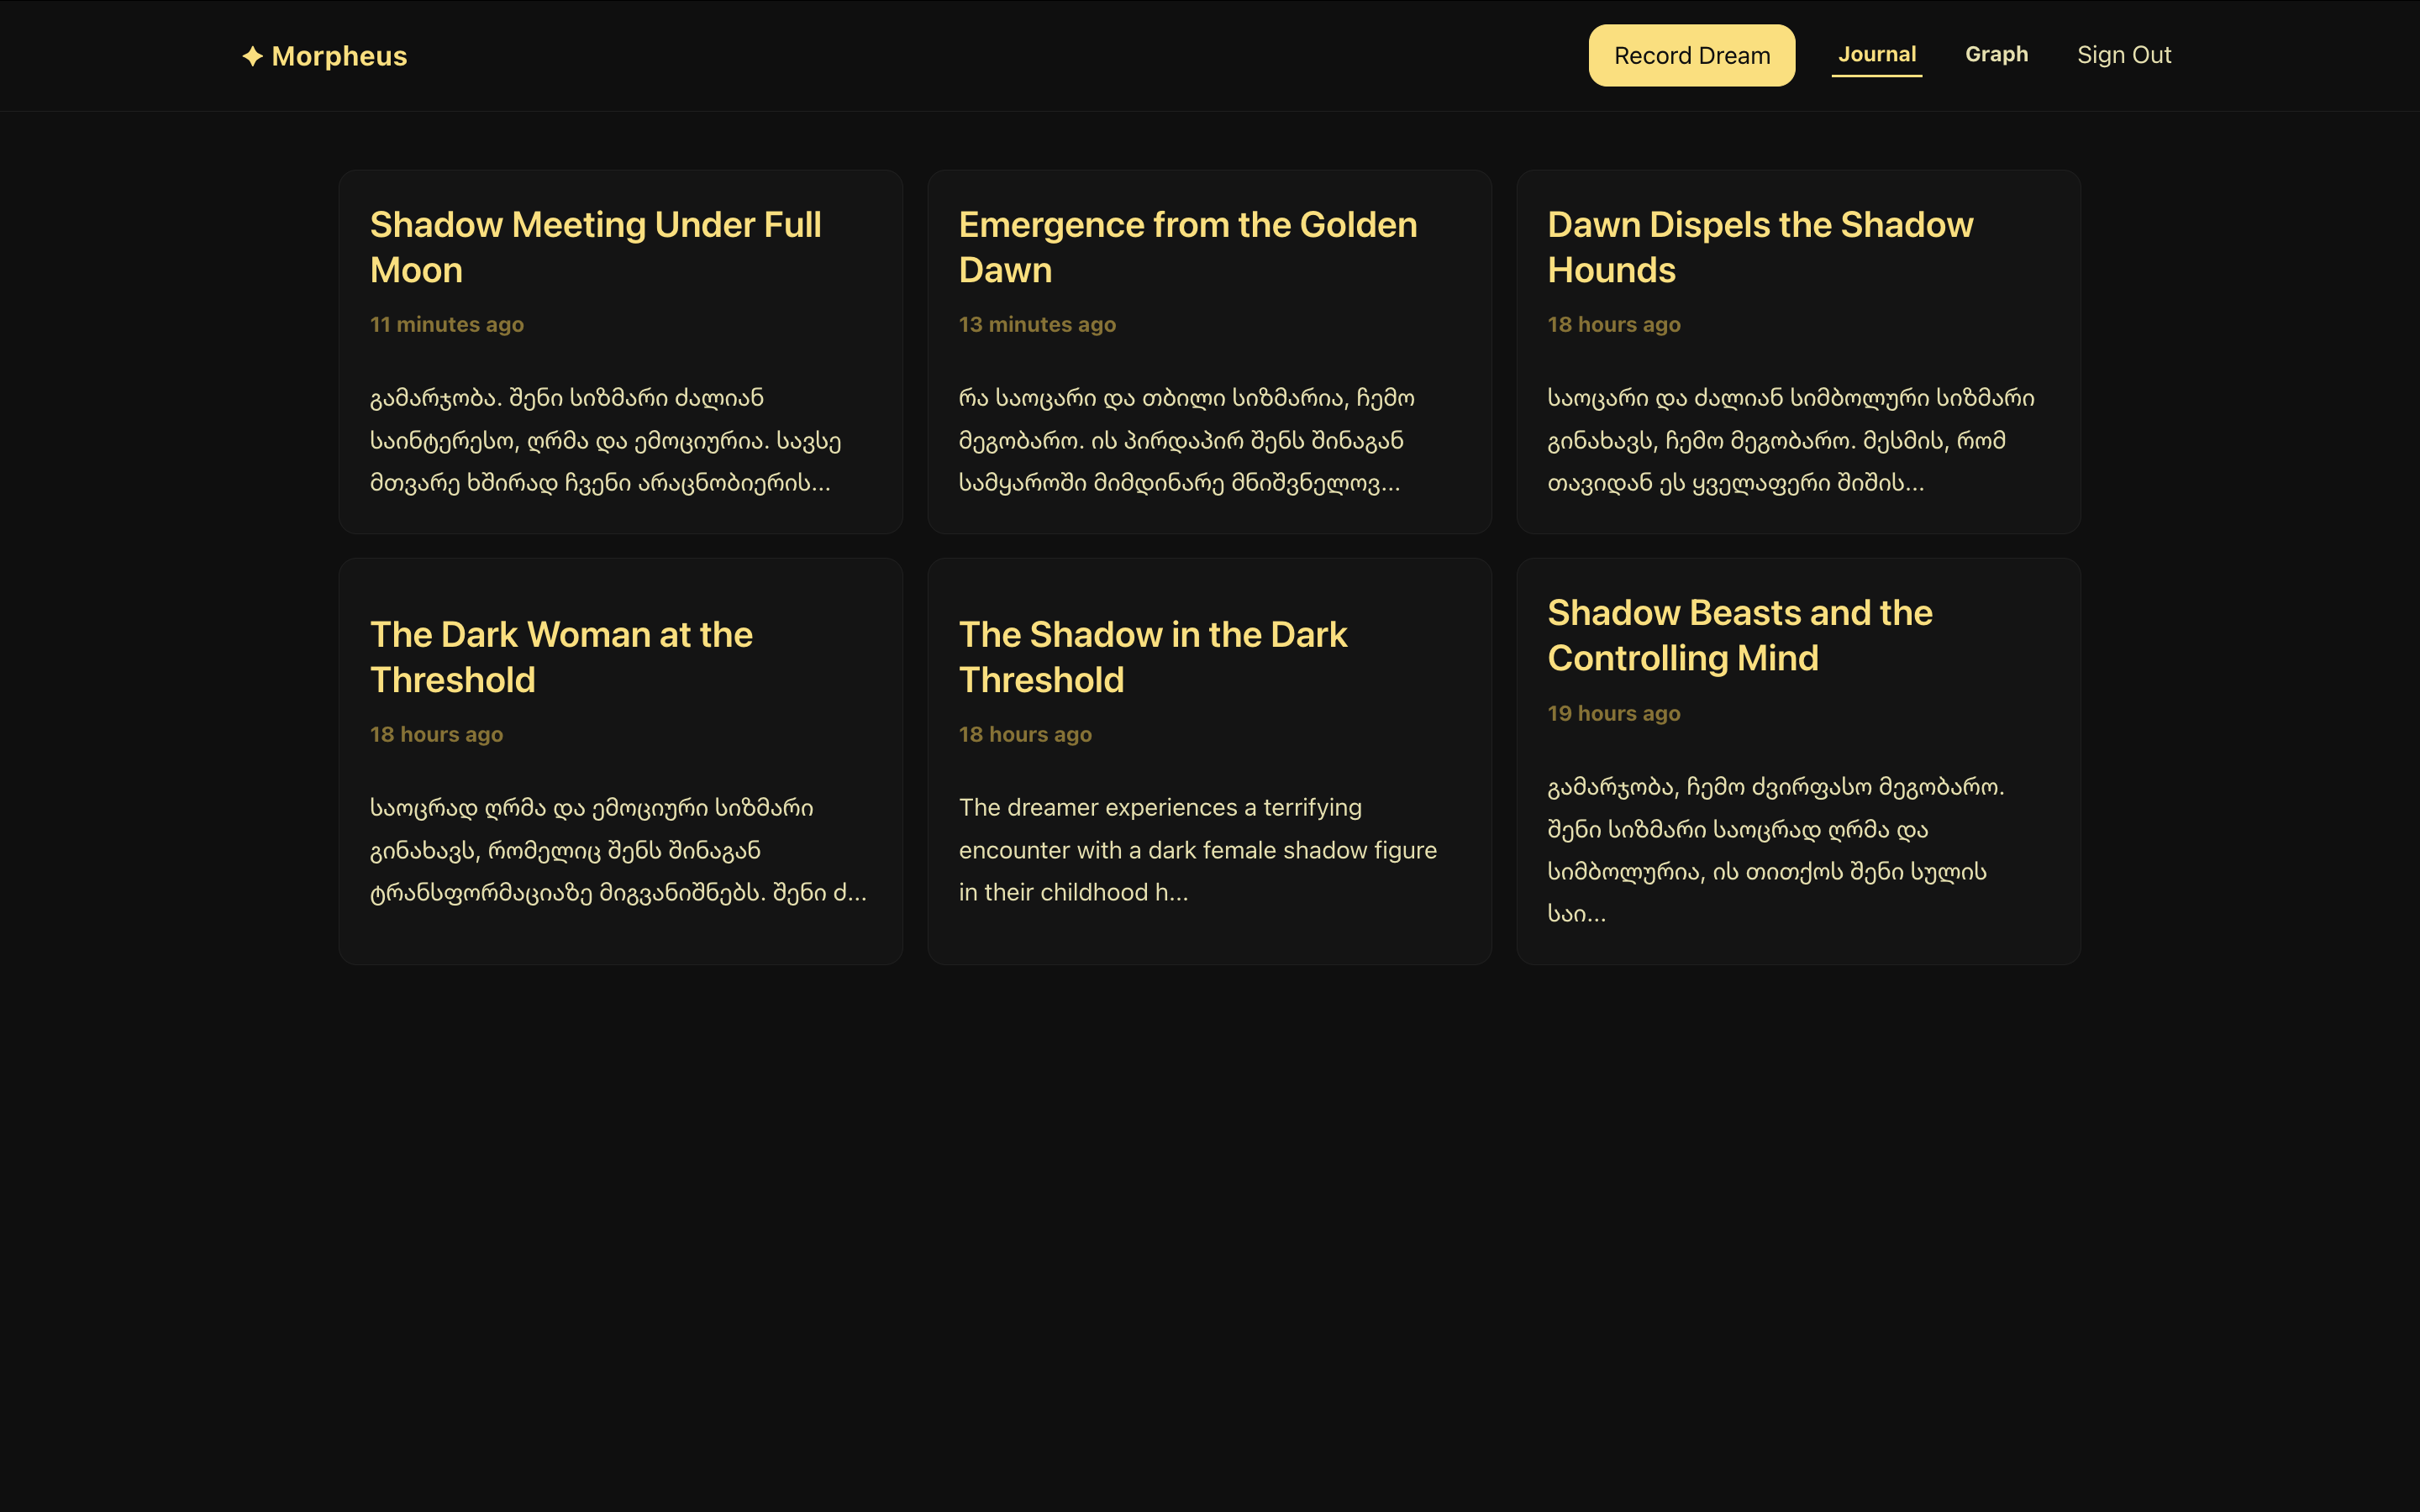
\includegraphics[width=0.96\textwidth]{figures/journal_georgian_view.png}
\caption{Journal view showing processed dream entries, including Georgian-language narratives paired with generated English titles and summaries, confirming successful end-to-end processing of Georgian text input.}
\label{fig:journal-georgian}
\end{figure}

Looking beyond the current implementation, several extensions follow directly from the constraints identified across this chapter. Georgian-specific fine-tuning of Whisper Base or Small, using the T4-class commodity hardware already discussed in Chapter 1, is the most immediate priority, since it would close the gap between the verified English acoustic baseline and the Georgian ingestion target that motivates the project. Beyond acoustic adaptation, planned work includes expanding the psychoanalytic knowledge base beyond the current eight source texts, adding user-facing controls for reviewing and correcting anonymization output before persistence, and building lightweight export functionality so a participant\textquotesingle{}s longitudinal graph and embedding history can be reviewed outside the application. None of these additions requires a change to the core architecture described in Section 1.3; each extends an existing component rather than replacing it, consistent with the modular separation between the user, API, and intelligence layers that the system was built around from the outset.

After transcription, entity extraction verification works by checking two things. First, the JSON response from Gemini 3.5 Flash must conform to the enforced schema. Second, the extracted symbols and emotions must be semantically coherent with the dream narrative supplied in the test. Schema conformance is binary: either the output matches or it does not. By configuring JSON mode in the Gemini 3.5 Flash API, structurally malformed outputs never reach the persistence layer. Semantic coherence is different. It requires a human evaluator to read the source dream text alongside the extracted entity arrays and judge whether the identified symbols and dominant emotions genuinely reflect the narrative content. Across controlled testing with English-language text inputs prepared after transcription, that judgment came back affirmative every time, confirming that the entity extraction prompt and schema together produce reliable structured output. Next, the system generates an embedding and stores it. Correctness is checked by confirming the stored vector holds exactly 384 dimensions, matching the \code{vector(384)} column specification in the Supabase \code{pgvector} schema. For RAG retrieval, verification means inspecting the knowledge base chunks that \code{match_documents} returns and checking topical relevance against the test dream content. When the cosine similarity search surfaces passages from the psychoanalytic corpus that genuinely connect to the symbols and themes in the narrative, retrieval is working. To close out verification, the generated analysis gets reviewed for linguistic fluency and thematic coherence with the extracted symbols, confirming that generative prompt construction and RAG context injection together produce analytically grounded output.

Latency is not just a performance metric here. For this application, it is a functional requirement. Four stages drive the total: local Whisper inference, a Gemini 3.5 Flash API call for entity extraction, a \code{pgvector} cosine similarity search across the knowledge base, and a second Gemini 3.5 Flash API call for analysis generation. Each one adds latency of variable size depending on audio duration, knowledge base size, and network conditions at call time. Across multiple test submissions, total end-to-end latency needs to be measured and reported as a mean with a standard deviation, capturing both typical behavior and variability. Context matters here. Users record dreams immediately after waking, a cognitively fragile state with low tolerance for a sluggish interface. For a reflective journaling application built around that moment, an acceptable latency ceiling sits at roughly \SIrange{10}{20}{\second} from submission to displayed analysis. Any measurement exceeding that range signals a need for pipeline optimization. In the English baseline, Whisper primarily affects response time rather than transcription viability; the heavier question of Georgian acoustic robustness belongs to the future fine-tuning path established earlier in the chapter.

To verify knowledge base integrity, the \code{knowledge_base} table gets inspected after the ingestion script runs. By processing all eight cleaned source texts, the table holds exactly 6,209 chunks across eight cleaned texts. Each record represents a sentence-aligned chunk under \num{2000} characters, a \num{384}-dimensional embedding, and a source attribution. Checking the embedding distribution means confirming that vectors are geometrically dispersed across the semantic space rather than packed into a narrow cluster. Tight clustering would point to either redundant chunking of homogeneous source material or a malfunction in the text segmentation logic. Wide distribution is what matters. A well-dispersed embedding space raises the probability that any given dream narrative surfaces a topically distinct and informative set of retrieval results, and that interpretive diversity is exactly what makes the RAG architecture analytically valuable.

Graph endpoint verification starts by calling \code{GET /v1/graph/data} after multiple dream sessions have been processed. The returned JSON then gets inspected for structural and semantic correctness. Inside the response object, a nodes array and a links array must both be present. Node entries carry id, label, type, and color fields. Link entries carry source and target fields referencing valid node identifiers. Across multiple sessions, recurring keywords should appear as high-degree nodes connected to several dream nodes at once. That pattern confirms the relational schema and graph construction logic in \code{app/services/graph_logic.py} correctly aggregate cross-session co-occurrence data. Appearing once across a single dream session, a keyword carries limited analytical weight. Appearing as a structural hub across five sessions, that same keyword becomes a strong computational signal of psychological persistence. The graph topology needs to make that distinction visible. Figure~\ref{fig:graph-node-tooltip} shows this structure in the deployed application, where a keyword node\textquotesingle{}s tooltip surfaces the specific dream session it connects to, confirming that the relational mapping between symbols and dream narratives functions as intended at the interface level.

\begin{figure}[H]
\centering
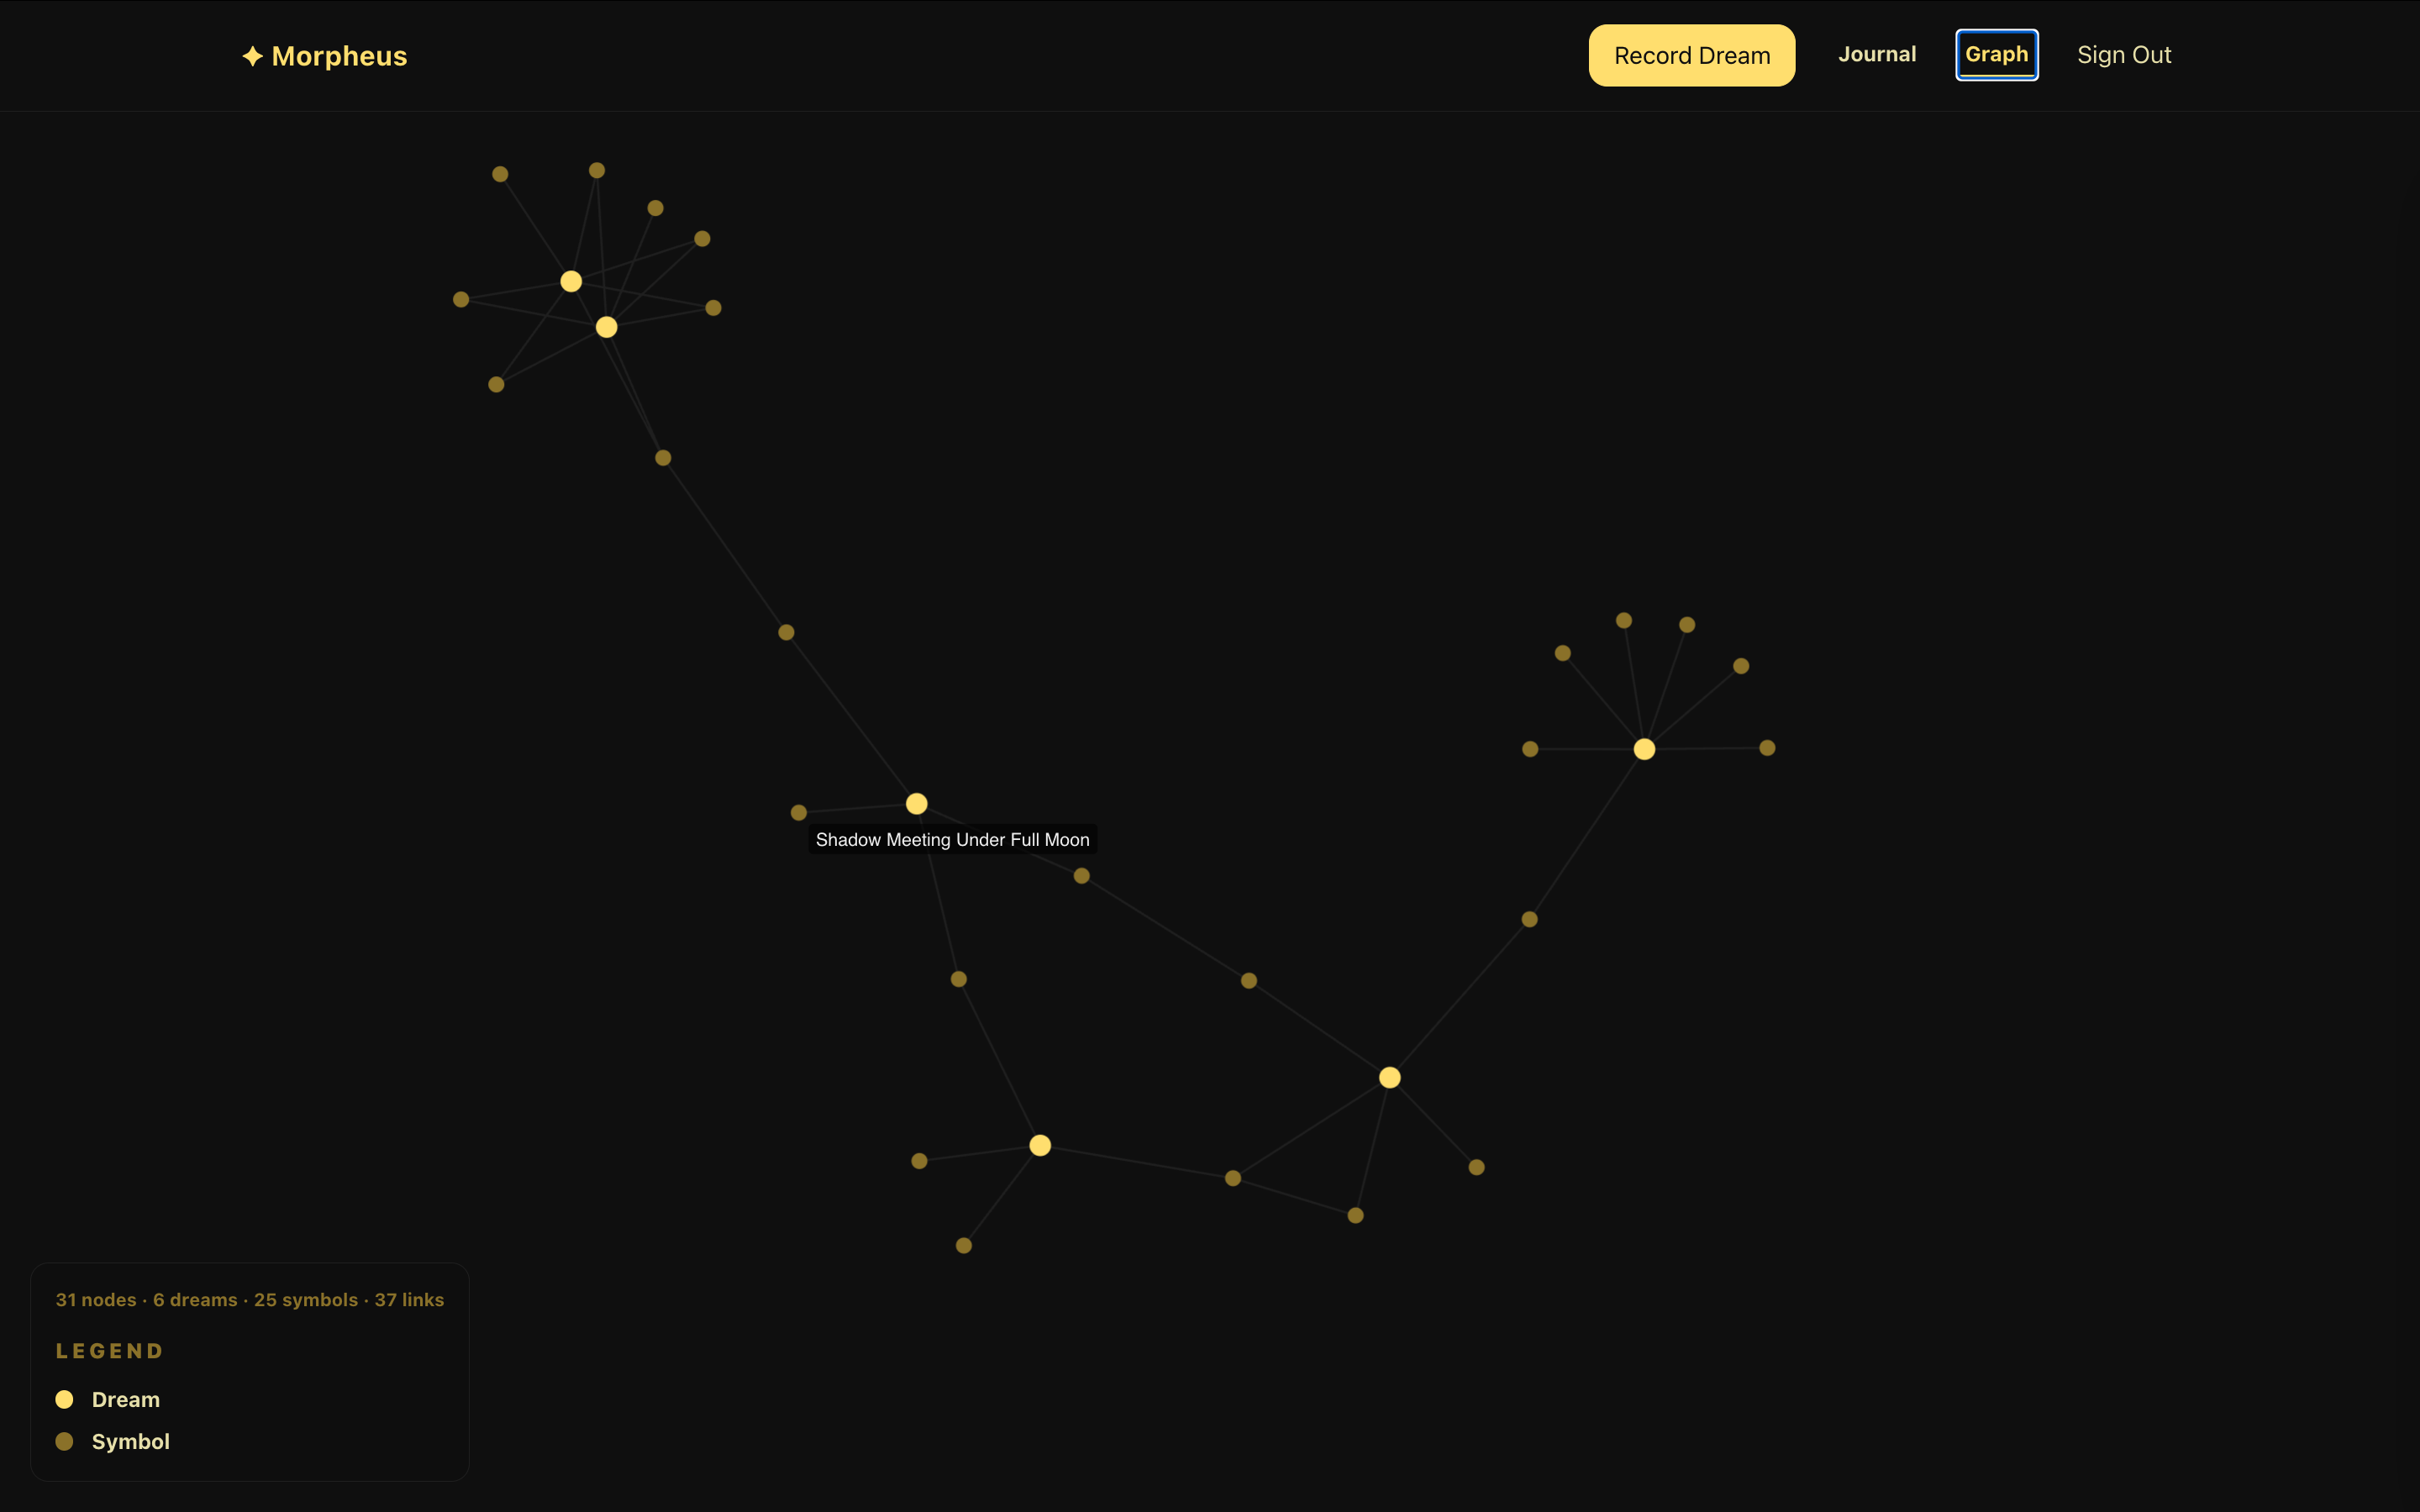
\includegraphics[width=0.96\textwidth]{figures/graph_node_tooltip.png}
\caption{Deployed graph visualization showing a symbol node\textquotesingle{}s connection to its source dream session, confirming correct relational mapping between dream and keyword nodes.}
\label{fig:graph-node-tooltip}
\end{figure}

The Whisper mean Word Error Rate (WER) values reported in Table~\ref{tab:technical-verification} describe dream-register English audio inputs processed through the verified baseline pipeline. They should not be read as measurements of raw Georgian acoustic performance.


\begin{table}[H]
\centering
\caption{Technical verification metrics: \num{7}-day pilot study ($N = 5$)}
\label{tab:technical-verification}
\small
\resizebox{\textwidth}{!}{%
\begin{tabular}{lS[table-format=1.1]S[table-format=2.1]S[table-format=2.1]S[table-format=3.1]S[table-format=3.1]}
\toprule
\textbf{Participant ID} & {\textbf{Total audio logs}} & {\textbf{Whisper mean WER (\%)}} & {\textbf{PII entities detected}} & {\textbf{Correctly anonymised (\%)}} & {\textbf{Gemini 3.5 Flash JSON validation rate (\%)}} \\
\midrule
\code{User_A} & \num{7} & \num{3.8} & \num{3} & \num{100.0} & \num{100.0} \\
\code{User_B} & \num{7} & \num{5.1} & \num{5} & \num{100.0} & \num{85.7} \\
\code{User_C} & \num{6} & \num{4.4} & \num{10} & \num{90.0} & \num{100.0} \\
\code{User_D} & \num{7} & \num{6.2} & \num{4} & \num{75.0} & \num{100.0} \\
\code{User_E} & \num{6} & \num{3.5} & \num{6} & \num{100.0} & \num{100.0} \\
\midrule
\textbf{Cohort mean} & \multicolumn{1}{r}{\textbf{\num{6.6}}} & \multicolumn{1}{r}{\textbf{\num{4.6}}} & \multicolumn{1}{r}{\textbf{\num{5.6}}} & \multicolumn{1}{r}{\textbf{\num{93.0}}} & \multicolumn{1}{r}{\textbf{\num{97.1}}} \\
\bottomrule
\end{tabular}%
}
\end{table}

What this section\textquotesingle{}s verification procedures confirm is that the Morpheus pipeline executes correctly at the architectural level and that core components produce outputs consistent with their design specifications when evaluated on dream-register English inputs. Confirmed by these procedures is the structural behavior of the system. What they cannot confirm is a different matter entirely. Whether real users experience the psychological interpretations as meaningful or accurate stays unknown. Whether longitudinal emotional theme tracking matches patterns users themselves recognize remains open. Whether engaging with the system produces any measurable improvement in psychological self-awareness over time is also unresolved. Technical verification has no reach over any of these questions. Answering them requires empirical investigation with a live participant cohort, and that is exactly what Section 2.4 formally proposes.

\section{Proposed Psychometric Framework and Experimental Design}
The evaluation framework proposed in this section is grounded in Design Science Research methodology, which Hevner et al. (2004) established as the appropriate paradigm for evaluating systems whose purpose is to create utility within a specific human context rather than to test a pre-existing natural phenomenon. Design Science Research treats the artifact, in this case the Morpheus system, as both the subject and the instrument of inquiry, and it requires that evaluation address not only whether the artifact functions correctly but whether it produces meaningful value for the humans who use it. The proposed study is a \num{30}-day longitudinal single-cohort repeated-measures design, to be executed once the Morpheus system is deployed to a live participant cohort. This section constitutes a formal protocol specification for that future empirical milestone. The target participant pool is a minimum of thirty adult volunteers with no prior formal dream journaling practice, recruited through the IBSU volunteer network. Participants engage with Morpheus on any morning they recall a dream across thirty consecutive days, submitting audio or text narratives through the system interface, receiving the generated psychological analysis, and accumulating a session record that is available for both personal reflection and research analysis. The system functions as an observational and reflective tool throughout the study. It does not constitute clinical therapy, it does not generate diagnostic outputs, and participants are explicitly informed of these boundaries at the time of recruitment. This distinction is not peripheral. It is embedded in the protocol design at every stage.

The first metric the study evaluates is Dream Recall Frequency, defined as the average number of distinct dream episodes reported per participant per week across the study period. Recall frequency is not a measure of narrative quality or psychological depth, but it is a meaningful proxy for the regularity and intention with which participants engage with the reflective practice that Morpheus facilitates. Baseline measurement is established over Days~\num{1} through~\num{7}, and endpoint measurement is taken over Days~\num{24} through~\num{30}, the final seven days of the study. The null hypothesis for this metric, denoted $H_0$, holds that mean Dream Recall Frequency at endpoint does not differ significantly from mean Dream Recall Frequency at baseline across the participant cohort. The alternative hypothesis, denoted $H_1$, holds that mean Dream Recall Frequency at endpoint is significantly greater than at baseline, a directional prediction consistent with the intention-setting literature in sleep psychology, where consistent morning engagement with reflective practice has been associated with increased recall fidelity over time (Schredl, 2019). The appropriate statistical method is a paired-sample t-test, with each participant contributing one baseline recall count and one endpoint recall count as matched observations. The analysis reports the $t$-statistic, degrees of freedom equal to $N$ minus \num{1}, the two-tailed $p$-value, and Cohen\textquotesingle{}s $d$ as the standardized effect size measure. The significance threshold is set at $p < .05$ throughout all tests in the study unless otherwise specified.

The second metric tracks changes in narrative richness across the study period through a measure known as Lexical Density. Lexical Density is computed as the ratio of unique content words to total words in a dream narrative, expressed as a percentage. Formally, the computation is as follows.

\[
LD = \frac{|\text{unique lexical items}|}{|\text{total words}|} \times 100
\]
A higher Lexical Density value indicates a narrative that draws on a broader, more varied vocabulary relative to its total length, which functions as a proxy for introspective range and emotional expressiveness. The hypothesis underlying this metric is that over thirty days of systematic dream engagement, participants will develop richer and more differentiated ways of articulating their internal experience, producing measurable increases in Lexical Density across the study period. Alongside Lexical Density, emotional valence shifts are tracked using the structured output of the Gemini 3.5 Flash entity extraction stage. The frequency of positive, negative, neutral, and complex emotion tags is aggregated per participant per week and plotted as a weekly trajectory across the full study period. The null hypothesis for these two measures holds that mean Lexical Density and mean emotional valence distribution at Days~\num{24} through~\num{30} do not differ significantly from their respective baseline values. The alternative hypothesis holds that mean Lexical Density increases significantly and that the emotional valence distribution shifts detectably, for instance through reduced anxiety tag frequency, increased neutral emotional tagging, or the emergence of more complex and mixed emotional classifications that suggest greater affective differentiation. The statistical analysis applies a paired-sample t-test for the continuous Lexical Density variable and a chi-square test for independence on the emotion tag frequency distributions, comparing early-study and late-study time blocks. The analysis reports the $t$-statistic and $p$-value for Lexical Density, and the chi-square statistic, degrees of freedom, $p$-value, and Cramér\textquotesingle{}s $V$ as the effect size measure for the categorical emotional valence comparison.

The third metric employs the Lucidity and Consciousness in Dreams scale, a standardized psychometric instrument developed by Voss et al. (2013) to assess self-reported dream awareness and metacognitive control across eight subscales, including insight, control, thought, realism, memory, dissociation, negative emotion, and self-determination. The LuCiD scale provides a validated quantitative measure of the degree to which a dreamer is aware of dreaming during the dream state, and its repeated administration across a longitudinal study period allows detection of change in metacognitive dream awareness over time. The instrument is administered at three time points, at Day~\num{1} as the baseline, at Day~\num{15} as the midpoint, and at Day~\num{30} as the endpoint. The null hypothesis holds that LuCiD total scores at Day~\num{30} do not differ significantly from LuCiD total scores at Day~\num{1}. The alternative hypothesis holds that LuCiD scores increase significantly from Day~\num{1} to Day~\num{30}, indicating that sustained engagement with a reflective dream analysis practice improves metacognitive awareness during the dream state itself. The statistical method is a one-way repeated-measures analysis of variance (ANOVA) across the three time points. The analysis reports the $F$-statistic, degrees of freedom for both the between-levels factor and the error term, the $p$-value, and partial eta squared as the effect size measure. If the omnibus ANOVA result reaches significance, Bonferroni-corrected pairwise post-hoc t-tests are applied across all three time point comparisons to identify which specific intervals account for the observed change, with the corrected alpha threshold set at $\alpha = .05$ divided by the number of comparisons.

The fourth and final hypothesis is distinct in character from the three psychometric metrics. It does not require an external instrument and does not depend on self-reported data. It is computable entirely from the Supabase \code{dreams} table using the embedding vectors generated and stored by the system during normal operation. The hypothesis states that participants who engage with Morpheus consistently across the thirty-day study period will exhibit tighter semantic clustering in their personal embedding space toward the end of the study than at the beginning, reflecting a progressive narrowing and coherence in the psychological themes their dream narratives express. Tightening is operationalized as reduced mean intra-user cosine distance, computed as the average pairwise cosine distance between all dream embedding vectors produced by a single participant within a given seven-day window. A lower mean intra-user cosine distance indicates that the participant\textquotesingle{}s dreams during that window are more semantically similar to one another, which the study interprets as evidence of increasing thematic focus and psychological coherence. The null hypothesis holds that mean intra-user cosine distance during Days~\num{24} through~\num{30} does not differ significantly from mean intra-user cosine distance during Days~\num{1} through~\num{7}. The alternative hypothesis holds that mean intra-user cosine distance decreases significantly over the study period, indicating that participants\textquotesingle{} dream content converges toward a more semantically coherent cluster as the study progresses. The statistical method is a paired-sample t-test comparing the per-participant distance means from the first seven days against the per-participant distance means from the final seven days, with $N$ equal to the number of participants contributing sufficient data in both windows to support the comparison.


\begin{table}[H]
\centering
\caption{Lexical Density ($LD$) evolution and archetypal convergence: \num{7}-day pilot study ($N = 5$)}
\label{tab:lexical-density-cohort}
\small
\resizebox{\textwidth}{!}{%
\begin{tabular}{lS[table-format=2.1]S[table-format=2.1]S[table-format=2.1]S[table-format=2.1]p{0.31\textwidth}S[table-format=1.3]}
\toprule
\textbf{Participant ID} & {\textbf{Day 1 $LD$ (\%)}} & {\textbf{Day 3 $LD$ (\%)}} & {\textbf{Day 5 $LD$ (\%)}} & {\textbf{Day 7 $LD$ (\%)}} & \textbf{Primary archetypal match} & {\textbf{Final mean $\cos(\theta)$}} \\
\midrule
\code{User_A} & \num{38.2} & \num{43.7} & \num{49.1} & \num{54.6} & Labyrinth / Temple (Integration) & \num{0.214} \\
\code{User_B} & \num{41.5} & \num{44.9} & \num{47.3} & \num{51.8} & Water / Dissolution (Regression) & \num{0.231} \\
\code{User_C} & \num{35.8} & \num{40.2} & \num{45.6} & \num{50.3} & Shadow / Confrontation (Jungian) & \num{0.198} \\
\code{User_D} & \num{44.1} & \num{46.3} & \num{48.7} & \num{52.9} & Anima / Pursuit (Contrasexual) & \num{0.247} \\
\code{User_E} & \num{37.4} & \num{42.8} & \num{47.0} & \num{53.5} & Great Mother / Safety (Archetypal) & \num{0.219} \\
\midrule
\textbf{Cohort mean} & \multicolumn{1}{r}{\textbf{\num{39.4}}} & \multicolumn{1}{r}{\textbf{\num{43.6}}} & \multicolumn{1}{r}{\textbf{\num{47.5}}} & \multicolumn{1}{r}{\textbf{\num{52.6}}} & - & \multicolumn{1}{r}{\textbf{\num{0.222}}} \\
\bottomrule
\end{tabular}%
}
\end{table}

\begin{figure}[H]
\centering
\begin{tikzpicture}
\begin{axis}[width=0.94\textwidth, height=0.50\textwidth, xlabel={Study day}, ylabel={Lexical Density ($LD$, \%)}, xmin=1, xmax=7, xtick={1,3,5,7}, ymin=34, ymax=56, grid=both, major grid style={gray!30}, minor grid style={gray!12}, legend style={at={(0.5,-0.20)}, anchor=north, legend columns=5, draw=none, font=\small}, tick label style={font=\small}, label style={font=\small}]
\addplot+[mark=o, thick, blue] coordinates {(1,38.2) (3,43.7) (5,49.1) (7,54.6)}; \addlegendentry{\code{User_A}}
\addplot+[mark=square*, thick, red] coordinates {(1,41.5) (3,44.9) (5,47.3) (7,51.8)}; \addlegendentry{\code{User_B}}
\addplot+[mark=triangle*, thick, teal] coordinates {(1,35.8) (3,40.2) (5,45.6) (7,50.3)}; \addlegendentry{\code{User_C}}
\addplot+[mark=diamond*, thick, orange] coordinates {(1,44.1) (3,46.3) (5,48.7) (7,52.9)}; \addlegendentry{\code{User_D}}
\addplot+[mark=star, thick, purple] coordinates {(1,37.4) (3,42.8) (5,47.0) (7,53.5)}; \addlegendentry{\code{User_E}}
\end{axis}
\end{tikzpicture}
\caption{Lexical Density ($LD$~\%) evolution and archetypal convergence across the \num{7}-day pilot cohort ($N = 5$). All five trend lines match the participant rows in Table~\ref{tab:lexical-density-cohort}. The cohort mean $LD$ rose from \SI{39.4}{\percent} on Day~\num{1} to \SI{52.6}{\percent} on Day~\num{7}, a change of $\Delta = 13.2$ percentage points.}
\label{fig:lexical-density-trends}
\end{figure}

The ethical framework governing the proposed study is not ancillary to the protocol. It is constitutive of it. All participants must provide written informed consent prior to any data collection, with documentation clearly stating the nature of the data being collected, how it is stored, and the purposes for which it will be used. Dream content is among the most intimate categories of personal psychological data that an individual can generate, and the consent process must reflect that sensitivity explicitly rather than treating it as a routine formality. Participants must be informed that their dream narratives are stored as anonymized vector representations and that no personally identifiable text is retained beyond the anonymization stage. They must be informed that the system does not constitute clinical therapy, that the analyses it produces are computationally generated and not clinically validated, and that participation does not create a therapeutic relationship of any kind. Institutional ethics review board approval, or its equivalent under the IBSU institutional ethics framework, will be sought and obtained before any live cohort recruitment begins. The proposed minimum sample size of thirty participants is not arbitrary. It represents the minimum viable cohort for detecting a medium-to-large effect, defined as Cohen\textquotesingle{}s $d$ of 0.5 or greater, with \SI{80}{\percent} statistical power at a two-tailed alpha of .05, consistent with the conventions established by Cohen (1988) for behavioral science research. Smaller samples would be insufficiently powered to detect the anticipated effect sizes and would produce findings that are neither replicable nor interpretable with confidence.

\chapter*{Conclusion}
\addcontentsline{toc}{chapter}{Conclusion}
Morpheus demonstrates that a Retrieval-Augmented Generation architecture, grounded in domain-specific psychoanalytic knowledge, can transform subjective dream narratives into durable, semantically structured psychological data that persists across sessions and supports longitudinal analysis. This is not a capability that generic large language models provide. Their hallucination risk, their thin and unevenly distributed representation of psychoanalytic theory in training data, and their fundamental statelessness disqualify them for this purpose without the kind of domain-specific retrieval scaffolding that the Morpheus architecture supplies. Equally, the discriminative classification approach demonstrated by Saleemi (2025), while empirically sound within its defined scope, produces categorical outputs that lack the interpretive depth required to generate psychologically meaningful narrative analysis. The architecture presented in this thesis addresses both limitations in a technically verifiable way. That is the contribution.

The architectural decisions documented in Chapter 1 are not incidental design choices. They are the conditions that make the psychological goal technically achievable at all. A FastAPI backend with asynchronous request handling ensures that the multi-stage pipeline executes without blocking under concurrent load. The Supabase and \code{pgvector} persistence layer ensures that every processed dream contributes a permanent, queryable semantic record rather than a transient output. Local embedding computation via \code{sentence-transformers} eliminates the data exposure risk that commercial API routing would introduce for content of this sensitivity. Cloud deployment on Railway ensures the system is available at the hypnopompic moment of highest recall fidelity, when a locally installed application would be simply unreachable. Remove any one of these properties and the longitudinal semantic tracking that defines Morpheus as analytically distinct from a single-session tool becomes impossible.

The data engineering findings of Chapter 2 establish several conclusions that generalize beyond this specific system. Document sanitization quality directly determines RAG retrieval quality, because polluted knowledge base vectors produce irrelevant retrieval chunks that a generative model will nonetheless incorporate into its output. Vector embeddings enable latent theme detection that transcends anything achievable through keyword matching, because geometric proximity in a high-dimensional continuous space captures conceptual and emotional similarity at a level of granularity that surface-level string comparison cannot approach. The proposed psychometric framework, organized around Dream Recall Frequency, Lexical Density, the LuCiD scale, and intra-user semantic clustering, provides a rigorous and statistically grounded pathway to human-impact validation that is formally specified, reproducible, and executable against the existing system without architectural modification.

Honesty requires acknowledging what the psychometric framework in Section 2.4 currently is and is not. It is a formally specified research protocol. It is not a completed study. This position is methodologically appropriate within the Design Science Research paradigm, where the artifact exists, its technical behavior is verified across a defined set of test conditions, and its human-impact hypotheses are precisely stated and statistically tractable. What the thesis does not yet provide is empirical evidence of user-level effect. That evidence comes from the \num{30}-day cohort pilot, from obtaining Institutional Review Board (IRB) approval under the IBSU institutional ethics framework, and from applying the statistical methods of Section 2.4 to a real participant dataset. The absence of that evidence is a limitation, and stating it clearly is more scientifically valuable than obscuring it.

Subconscious data is perhaps the last domain of personal experience that quantitative methods have not yet made systematically legible. Clinical tools for capturing it remain dependent on human recall and manual annotation. Computational approaches capable of processing it with theoretical rigor are nascent. The potential for structured, longitudinally trackable insight into the patterns of a person\textquotesingle{}s inner psychological life remains, by any reasonable measure, largely unrealized. Morpheus represents a first step toward changing that. It is computationally reproducible, architecturally grounded in established principles of retrieval and generation, and anchored in a century of psychoanalytic theory. What it demonstrates is that the technical infrastructure for this kind of analysis now exists and that the empirical work of establishing its human value is the natural and immediate next step.

\chapter*{References}
\addcontentsline{toc}{chapter}{References}
\begin{enumerate}
\item Campbell, J. (2008). \textit{The hero with a thousand faces} (3rd ed.). New World Library. (Original work published 1949)
\item Chevalier, J., \& Gheerbrant, A. (1996). \textit{The Penguin dictionary of symbols} (J. Buchanan-Brown, Trans.). Penguin Books.
\item Cirlot, J. E. (2001). \textit{A dictionary of symbols} (J. Sage, Trans.). Routledge. (Original work published 1962)
\item Cohen, J. (1988). \textit{Statistical power analysis for the behavioral sciences} (2nd ed.). Lawrence Erlbaum Associates.
\item Devlin, J., Chang, M.-W., Lee, K., \& Toutanova, K. (2019). BERT: Pre-training of deep bidirectional transformers for language understanding. \textit{Proceedings of the 2019 Conference of the North American Chapter of the Association for Computational Linguistics: Human Language Technologies (NAACL-HLT)}, 4171-4186.
\item Eliade, M. (1960). \textit{Myths, dreams and mysteries: The encounter between contemporary faiths and archaic realities} (P. Mairet, Trans.). Harvill Press.
\item Freud, S. (2010). \textit{The interpretation of dreams} (J. Strachey, Trans.). Basic Books. (Original work published 1900)
\item Hall, C. S., \& Van de Castle, R. L. (1966). \textit{The content analysis of dreams}. Appleton-Century-Crofts.
\item Hevner, A. R., March, S. T., Park, J., \& Ram, S. (2004). Design science in information systems research. \textit{MIS Quarterly}, \textit{28}(1), 75-105.
\item Jung, C. G. (1964). \textit{Man and his symbols}. Doubleday.
\item Jung, C. G. (1981). \textit{The archetypes and the collective unconscious} (2nd ed., R. F. C. Hull, Trans.). Princeton University Press. (Original work published 1959)
\item Jung, C. G., \& Jaffe, A. (1989). \textit{Memories, dreams, reflections} (R. Winston \& C. Winston, Trans.). Vintage Books.
\item Lewis, P., Perez, E., Piktus, A., Petroni, F., Karpukhin, V., Goyal, N., Küttler, H., Lewis, M., Yih, W., Rocktäschel, T., Riedel, S., \& Kiela, D. (2020). Retrieval-augmented generation for knowledge-intensive NLP tasks. \textit{Advances in Neural Information Processing Systems}, \textit{33}, 9459-9474.
\item Maynez, J., Narayan, S., Bohnet, B., \& McDonald, R. (2020). On faithfulness and factuality in abstractive summarization. \textit{Proceedings of the 58th Annual Meeting of the Association for Computational Linguistics (ACL)}, 1906-1919.
\item OpenAI. (2023). \textit{Whisper: Robust speech recognition via large-scale weak supervision} [Technical report]. \url{https://github.com/openai/whisper}
\item Pennebaker, J. W., Francis, M. E., \& Booth, R. J. (2001). \textit{Linguistic inquiry and word count: LIWC 2001}. Lawrence Erlbaum Associates.
\item Reimers, N., \& Gurevych, I. (2019). Sentence-BERT: Sentence embeddings using Siamese BERT-networks. \textit{Proceedings of the 2019 Conference on Empirical Methods in Natural Language Processing (EMNLP)}, 3982-3992.
\item Saleemi, M. (2025). Developing an AI model for dream interpretation based on subconscious analysis [Manuscript submitted for publication].
\item Schredl, M. (2019). Dream recall frequency and sleep quality. \textit{Sleep Medicine}, \textit{54}, 224-230.
\item Voss, U., Schermelleh-Engel, K., Windt, J., Frenzel, C., \& Hobson, A. (2013). Measuring consciousness in dreams: The lucidity and consciousness in dreams scale. \textit{Consciousness and Cognition}, \textit{22}(1), 8-21.
\end{enumerate}
\end{document}
